\documentclass[12pt]{report}
%\geometry{landscape}                % Activate for for rotated page geometry
%\usepackage[parfill]{parskip}    % Activate to begin paragraphs with an empty line rather than an indent
\usepackage{graphicx, amsmath, amssymb,epstopdf,stmaryrd,fancyhdr,fullpage,multicol,mathrsfs,algorithm, algorithmic,natbib,url,oz}
\DeclareGraphicsRule{.tif}{png}{.png}{`convert #1 `dirname #1`/`basename #1 .tif`.png}

%\usepackage[left=0.9in,top=0.9in,right=0.9in,bottom=0.8in]{geometry}
%\geometry{letterpaper}  

%%%%%DEFINITIONS%%%%%

% for the problems
\newcommand{\exercise}[1]{\subsubsection*{Exercise {#1}}}
\newcommand{\solution}{\subsubsection*{Solution}}

\newtheorem{definition}{Definition}
\newtheorem{theorem}{Theorem}
\newtheorem{lemma}{Lemma}

%common sets
\newcommand{\N}{\mathbb{N}}
\newcommand{\Z}{\mathbb{Z}}
\newcommand{\Q}{\mathbb{Q}}
\newcommand{\R}{\mathbb{R}}
\newcommand{\C}{\mathbb{C}}
\newcommand{\B}{\mathbb{B}}

%other math symbols
\newcommand{\Ker}{\mbox{ Ker }}
\newcommand{\Mod}{\mbox{ mod }}
\newcommand{\Var}{\mbox{ Var}}
\newcommand{\D}{\mbox{d}}
\newcommand\independent{\protect\mathpalette{\protect\independenT}{\perp}}
\def\independenT#1#2{\mathrel{\rlap{$#1#2$}\mkern3mu{#1#2}}}

% category theory
\newcommand{\Ob}{\textrm{Ob}}
\newcommand{\Bool}{\textbf{Bool}}
\newcommand{\Cost}{\textbf{Cost}}

\newcommand{\mcA}{\mathcal{A}}
\newcommand{\mcB}{\mathcal{B}}
\newcommand{\mcC}{\mathcal{C}}
\newcommand{\mcD}{\mathcal{D}}
\newcommand{\mcE}{\mathcal{E}}
\newcommand{\mcF}{\mathcal{F}}
\newcommand{\mcG}{\mathcal{G}}
\newcommand{\mcH}{\mathcal{H}}
\newcommand{\mcI}{\mathcal{I}}
\newcommand{\mcJ}{\mathcal{J}}
\newcommand{\mcK}{\mathcal{K}}
\newcommand{\mcL}{\mathcal{L}}
\newcommand{\mcM}{\mathcal{M}}
\newcommand{\mcN}{\mathcal{N}}
\newcommand{\mcO}{\mathcal{O}}
\newcommand{\mcP}{\mathcal{P}}
\newcommand{\mcQ}{\mathcal{Q}}
\newcommand{\mcR}{\mathcal{R}}
\newcommand{\mcS}{\mathcal{S}}
\newcommand{\mcT}{\mathcal{T}}
\newcommand{\mcU}{\mathcal{U}}
\newcommand{\mcV}{\mathcal{V}}
\newcommand{\mcW}{\mathcal{W}}
\newcommand{\mcX}{\mathcal{X}}
\newcommand{\mcY}{\mathcal{Y}}
\newcommand{\mcZ}{\mathcal{Z}}

\title{Applied Category Theory Problems}
\author{April Shen \& Alex Root}

\begin{document}
\maketitle

\chapter{Generative Effects}

\exercise{1.1}
A function $f:\R\to\R$ is said to be
\begin{itemize}
    \item \emph{order-preserving} if $x \leq y$ implies $f(x) \leq f(y)$, for all $x, y \in \R$
    \item \emph{metric-preserving} if $|x-y|=|f(x)-f(y)|$
    \item \emph{addition-preserving} if $f(x+y)=f(x)+f(y)$
\end{itemize}
For each of the three properties defined above—call it \emph{foo}—find an $f$ that is \emph{foo}-preserving and an example of an $f$ that is not \emph{foo}-preserving.

\solution
$f(x) = x$ is order-, metric-, and addition-preserving.  $f(x) = x^2$ is none of these.

\exercise{1.4}
See book.

\solution
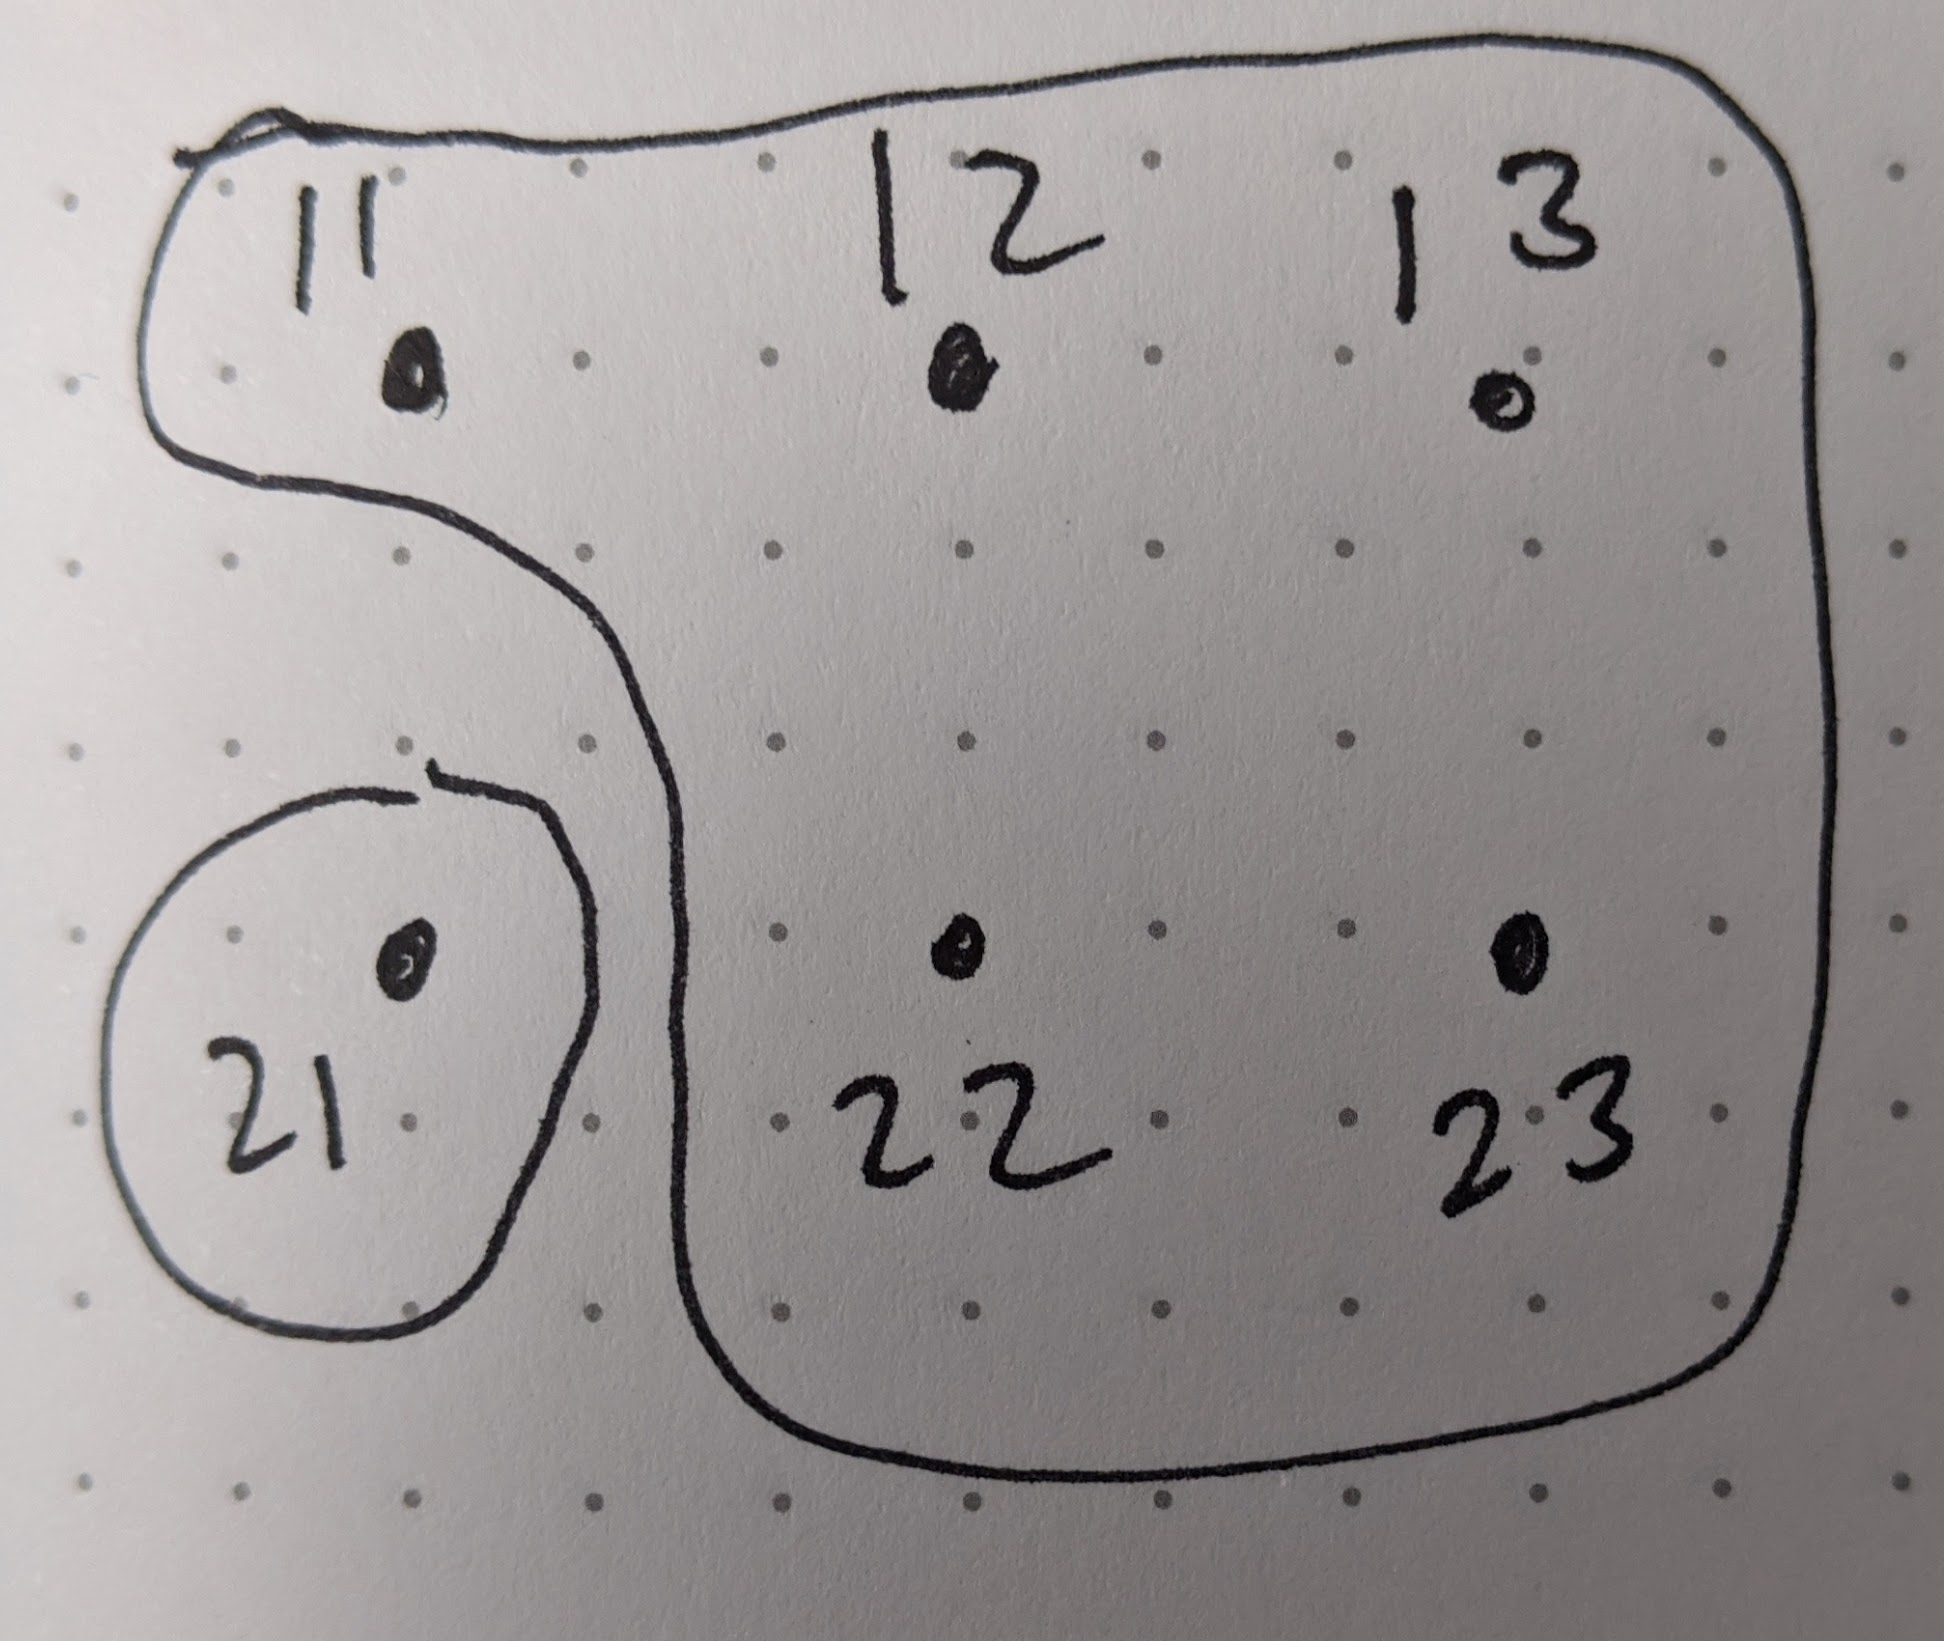
\includegraphics[width=0.5\linewidth]{images/1-4.jpg}

\exercise{1.6, 1.7, 1.10}
Discussed in person

\exercise{1.11}
Let $A = \{h, 1\}$ and $B = \{1, 2, 3\}$.

\solution
\begin{enumerate}
    \item The subsets of $B$ are $\varnothing, \{1\}, \{2\}, \{3\}, \{1, 2\}, \{1, 3\}, \{2, 3\}, \{1,2,3\}$.
    \item For example, $\{1, 2\} \cup \{2\} = \{1, 2\}$.
    \item $A\times B = \{(h, 1), (h, 2), (h, 3), (1, 1), (1, 2), (1, 3)\}$
    \item $A\sqcup B = \{h_A, 1_A, 1_B, 2_B, 3_B\}$
    \item $A\cup B = \{h, 1, 2, 3, 4\}$
\end{enumerate}

\exercise{1.16}
Suppose that $A$ is a set and $\{A_p\}_{p\in P}$ and $\{A'_{p'}\}_{p'\in P'}$ are two partitions of $A$ such that for each $p\in P$ there exists a $p'\in P'$ with $A_p = A'_{p'}$.
\begin{enumerate}
    \item Show that for each $p\in P$ there is at most one $p'\in P'$ such that $A_p= A'_{p'}$.
    \item Show that for each $p'\in P'$ there is a $p\in P$ such that $A_p = A'_{p'}$.
\end{enumerate}

\solution
\begin{enumerate}
    \item If there are distinct $p'_1, p'_2\in P'$ such that $A_p=A'_{p'_1}$ and $A_p=A'_{p'_2}$, then by transitivity $A'_{p'_1}=A'_{p'_2}$ which means that $p'_1=p'_2$ as $P'$ is a partition.
    \item Let $a\in A'_{p'_1}$.  Then we must have that $a\in A_p$ for some $p$.  We will show that this $A_p$ is the desired one.  There must exist $p'_2$ such that $A_p=A'_{p'_2}$.   So $a \in A'_{p'_2}$ and $a\in A'_{p'_1}$.  So $A'_{p'_1} = A'_{p'_2} = A_p$ as we wanted.
\end{enumerate}

\exercise{1.17}
See book.

\solution
$(11, 11), (12, 12), (13,13), (21,21), (22,22), (23,23), (11, 12), (12, 11), (22, 23), (23,22)$

\exercise{1.20}
Suppose that $\sim$ is an equivalence relation on a set $A$, and let $P$ be the set of $(\sim)$-closed and $(\sim)$-connected subsets $\{A_p\}_{p\in P}$.
\begin{enumerate}
    \item Show that each part $A_p$ is nonempty.
    \item Show that if $p\neq q$ i.e. $A_p \neq A_q$, then $A_p\cap A_q = \varnothing$.
    \item Show that $A = \bigcup_{p\in P} A_p$.
\end{enumerate}

\solution
\begin{enumerate}
    \item Since each $A_p$ is $(\sim)$-connected, by definition $A_p$ must be nonempty.
    \item Suppose $a\in A_p \cap A_q$. Then for any $b\in A_p$, we know $b\sim a$, hence since $A_q$ is $(\sim)$-closed we know $b\in A_q$.  Similarly for any $b\in A_q$.  Hence $A_p = A_q$.
    \item Clearly $\bigcup A_p\subseteq A$.  Suppose $a\in A$.  Then let $X=\{b\ |\ a\sim b, b\in A\}$.  $X$ is closed as the equivalence relation is reflexive and connected as it is transitive, so $X$ a set in $\{A_p\}$ and $A\subseteq \bigcup A_p$.
\end{enumerate}

\exercise{1.24}
Discussed in person

\exercise{1.25}
Suppose that $A$ is a set and $f : A \to\varnothing$  is a function to the empty set. Show that $A$ is empty.

\solution
Suppose there is some $a\in A$.  Then we must have $f(a)\in\varnothing$ which is clearly not possible.

\exercise{1.27, 1.38, 1.40, 1.41, 1.42, 1.44}
Discussed in person

\exercise{1.46}
Write down the numbers $1,2,\dots,10$ and draw an arrow $a\to b$ if $a$ divides perfectly into $b$. Is it a total order?

\solution
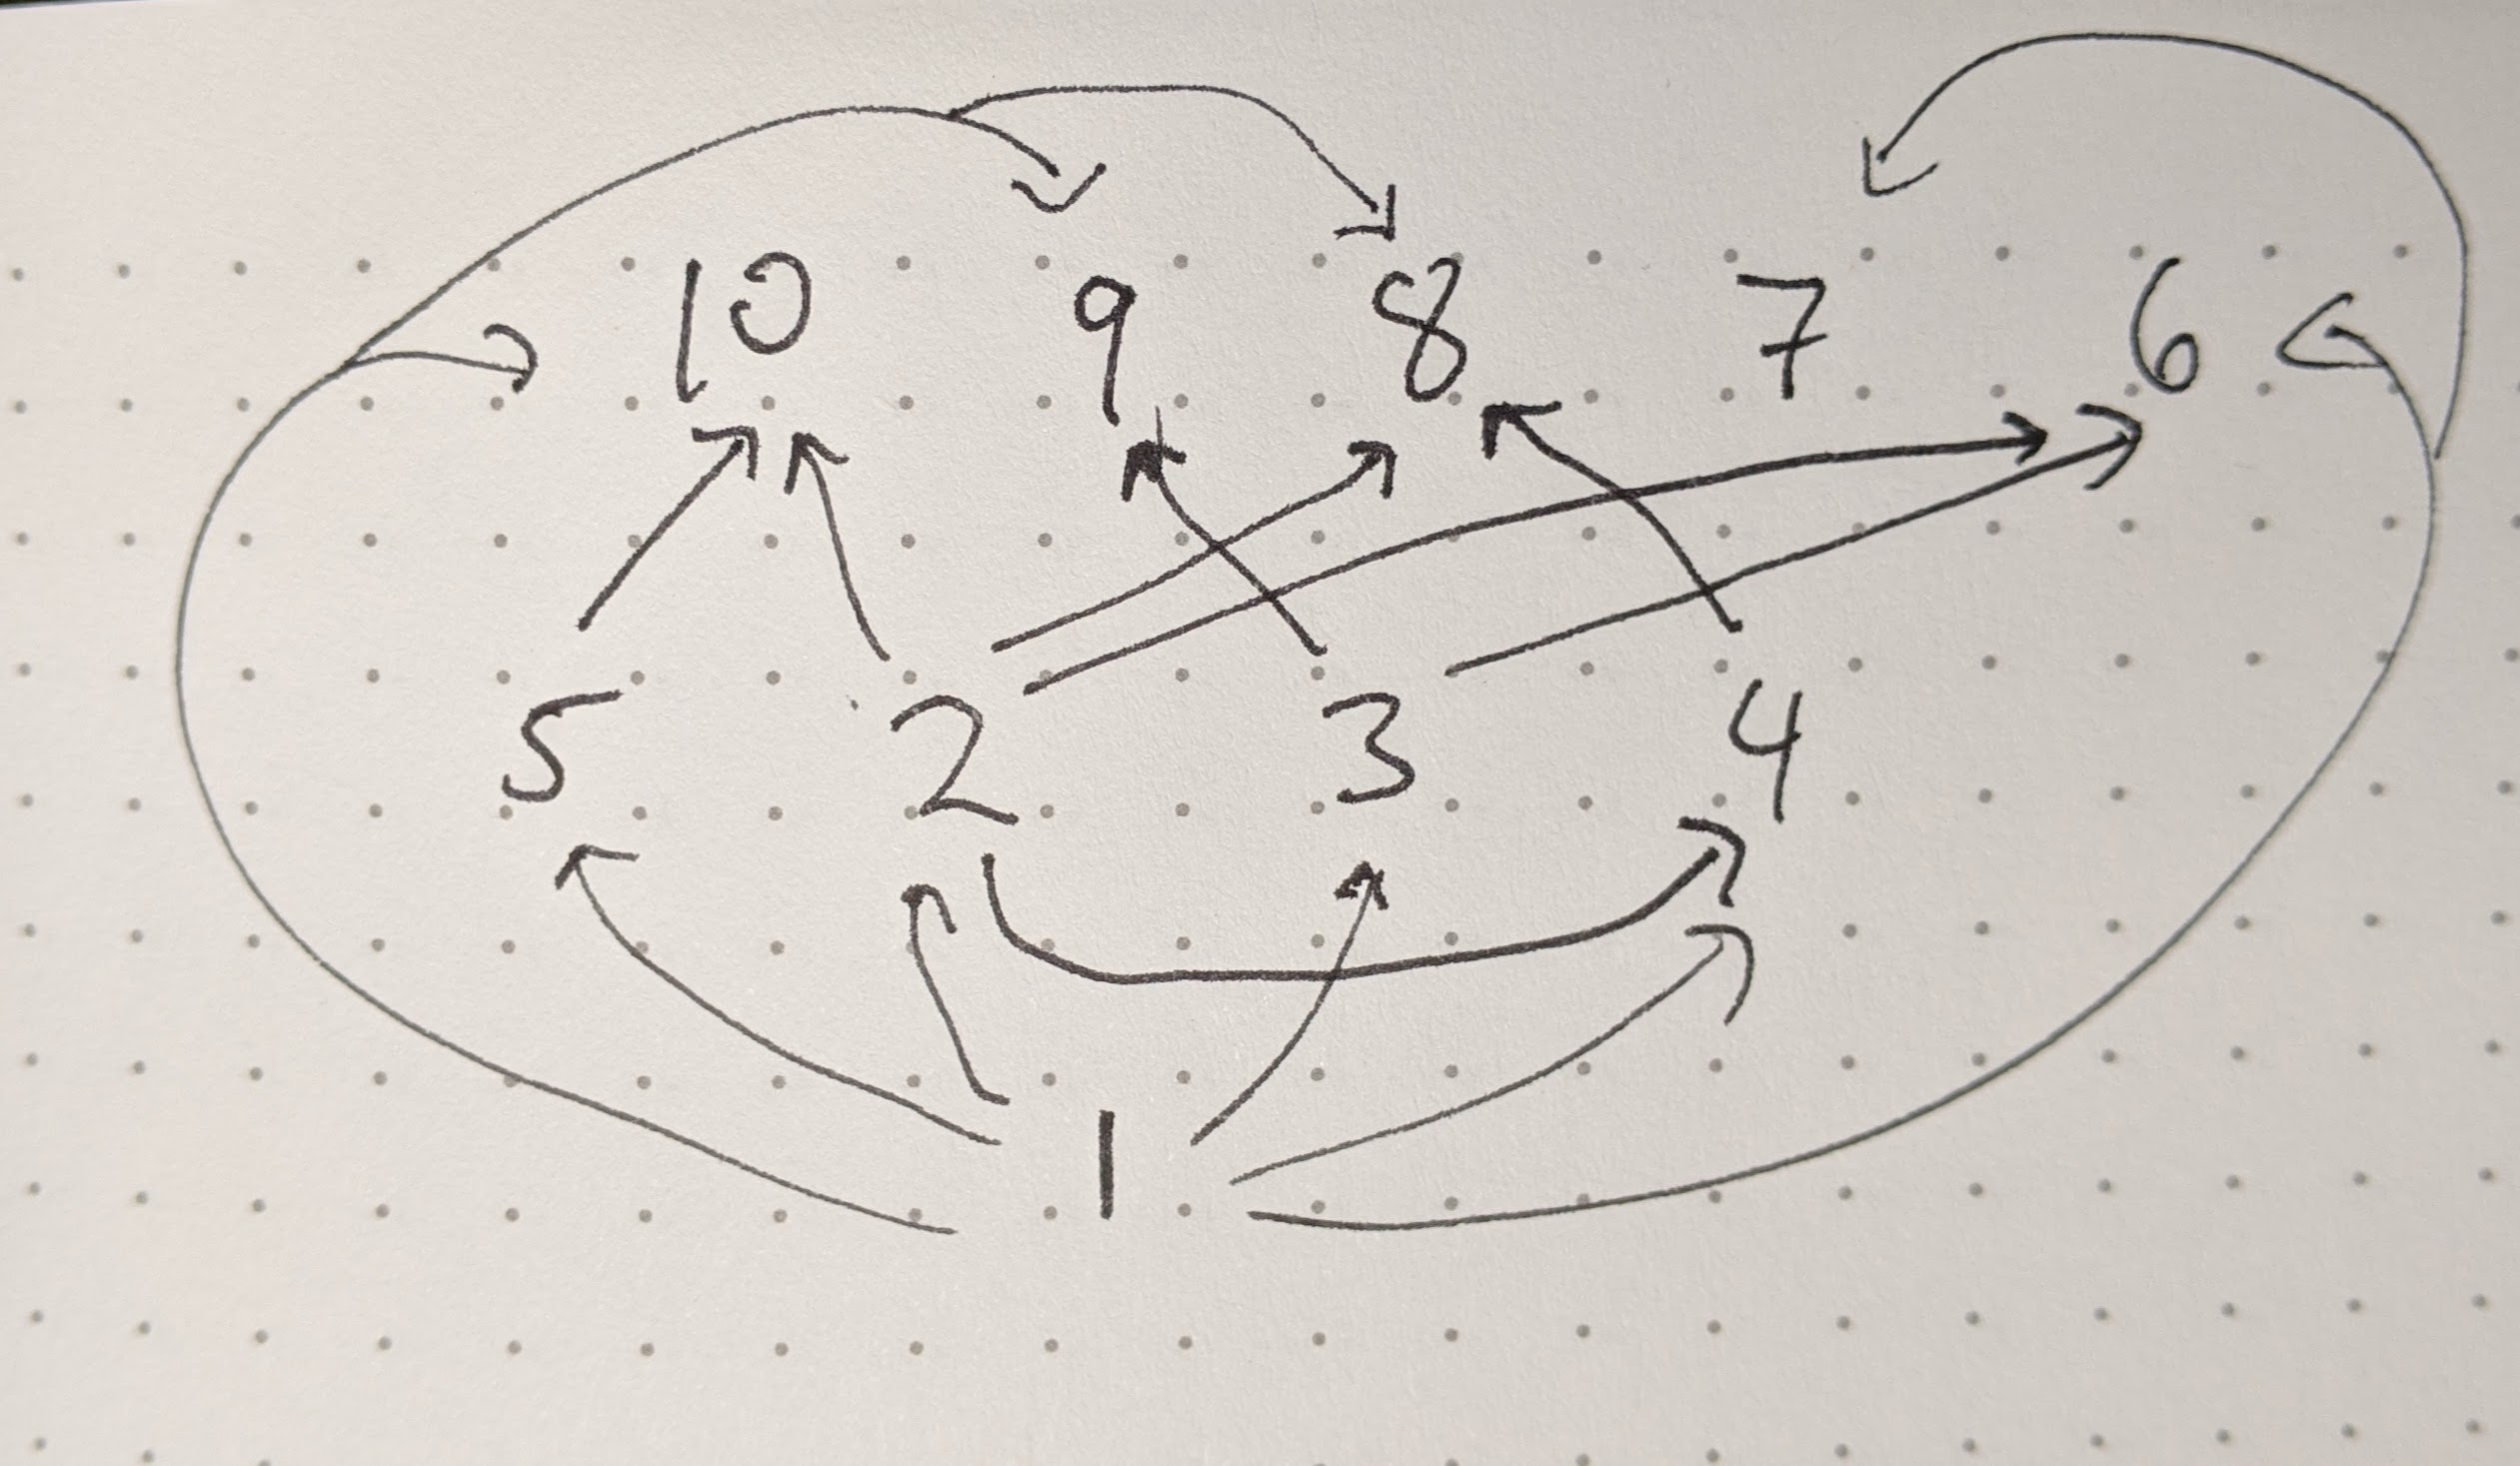
\includegraphics[width=0.5\linewidth]{images/1-46.jpg}

This isn't a total order, as for example we neither have $2|7$ or $7|2$.

\exercise{1.48}
Is the usual $\leq$ ordering on the set $\R$ of real numbers a total order?

\solution
Yes: for any $x,y\in\R$, we have $x\leq y$ or $y\leq x$.

\exercise{1.51}
Discussed in person

\exercise{1.53}
For any set $S$ there is a coarsest partition, having just one part. What surjective function does it correspond to?
There is also a finest partition, where everything is in its own partition. What surjective function does it correspond to?

\solution
Let $f:S\to\{\bullet\}$ be the unique function that sends every element of $S$ to $\bullet$.  This is a surjection corresponding to the coarsest partition, i.e. where every element is in the same set.

Let $f: S\to S$ be the identity function.  This is a surjection corresponding to the finest partition, i.e. where every element is in its own set.

\exercise{1.55}
Prove that the preorder of upper sets on a discrete preorder on a set $X$ is simply the power set $P(X)$.

\solution
Clearly the set of upper sets $U(X)$ is a subset of the power set $P(X)$.

Let $Y\subseteq X$.  We know $\varnothing$ is an upper set, so let $y\in Y$. Then since the preorder is discrete, the only element in $X$ greater than $y$ is y itself, which is in $Y$.  This holds for any $y\in Y$ so $Y$ is an upper set.  Note that the ordering on both $U(X)$ and $P(X)$ is the same, i.e. $\subseteq$.

\exercise{1.57}
See book.

\solution
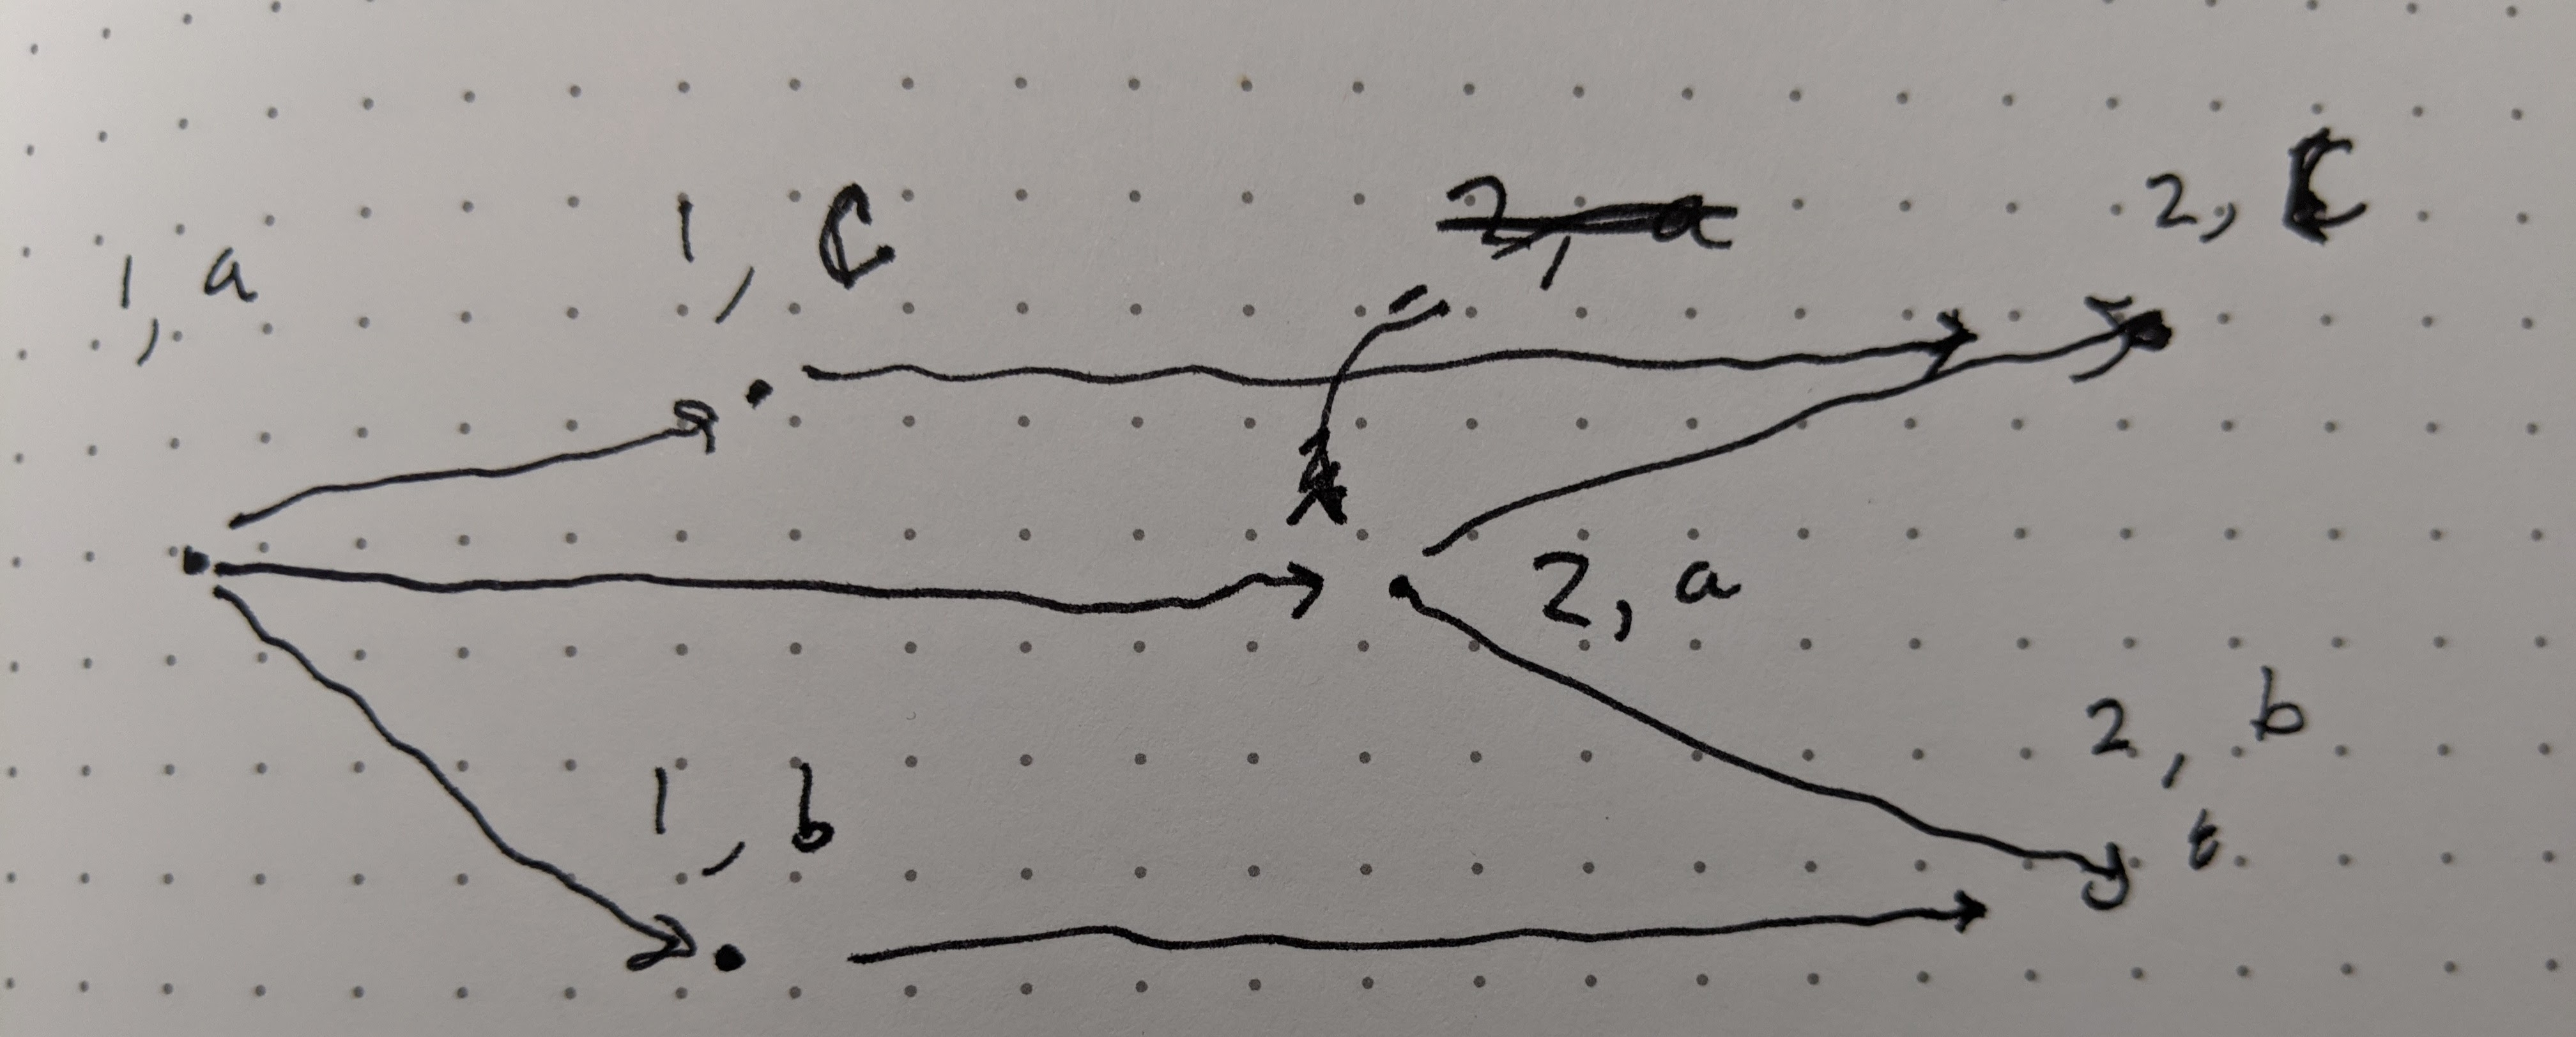
\includegraphics[width=0.5\linewidth]{images/1-57.jpg}

\exercise{1.63}
Let $X = \{0, 1, 2\}$.
\begin{enumerate}
    \item Draw the Hasse diagram for $P(X)$.
    \item Draw the Hasse diagram for the preorder $0 \leq 1 \leq 2 \leq 3$.
    \item Draw the cardinality map $|\cdot|$ as dashed lines between them
\end{enumerate}

\solution
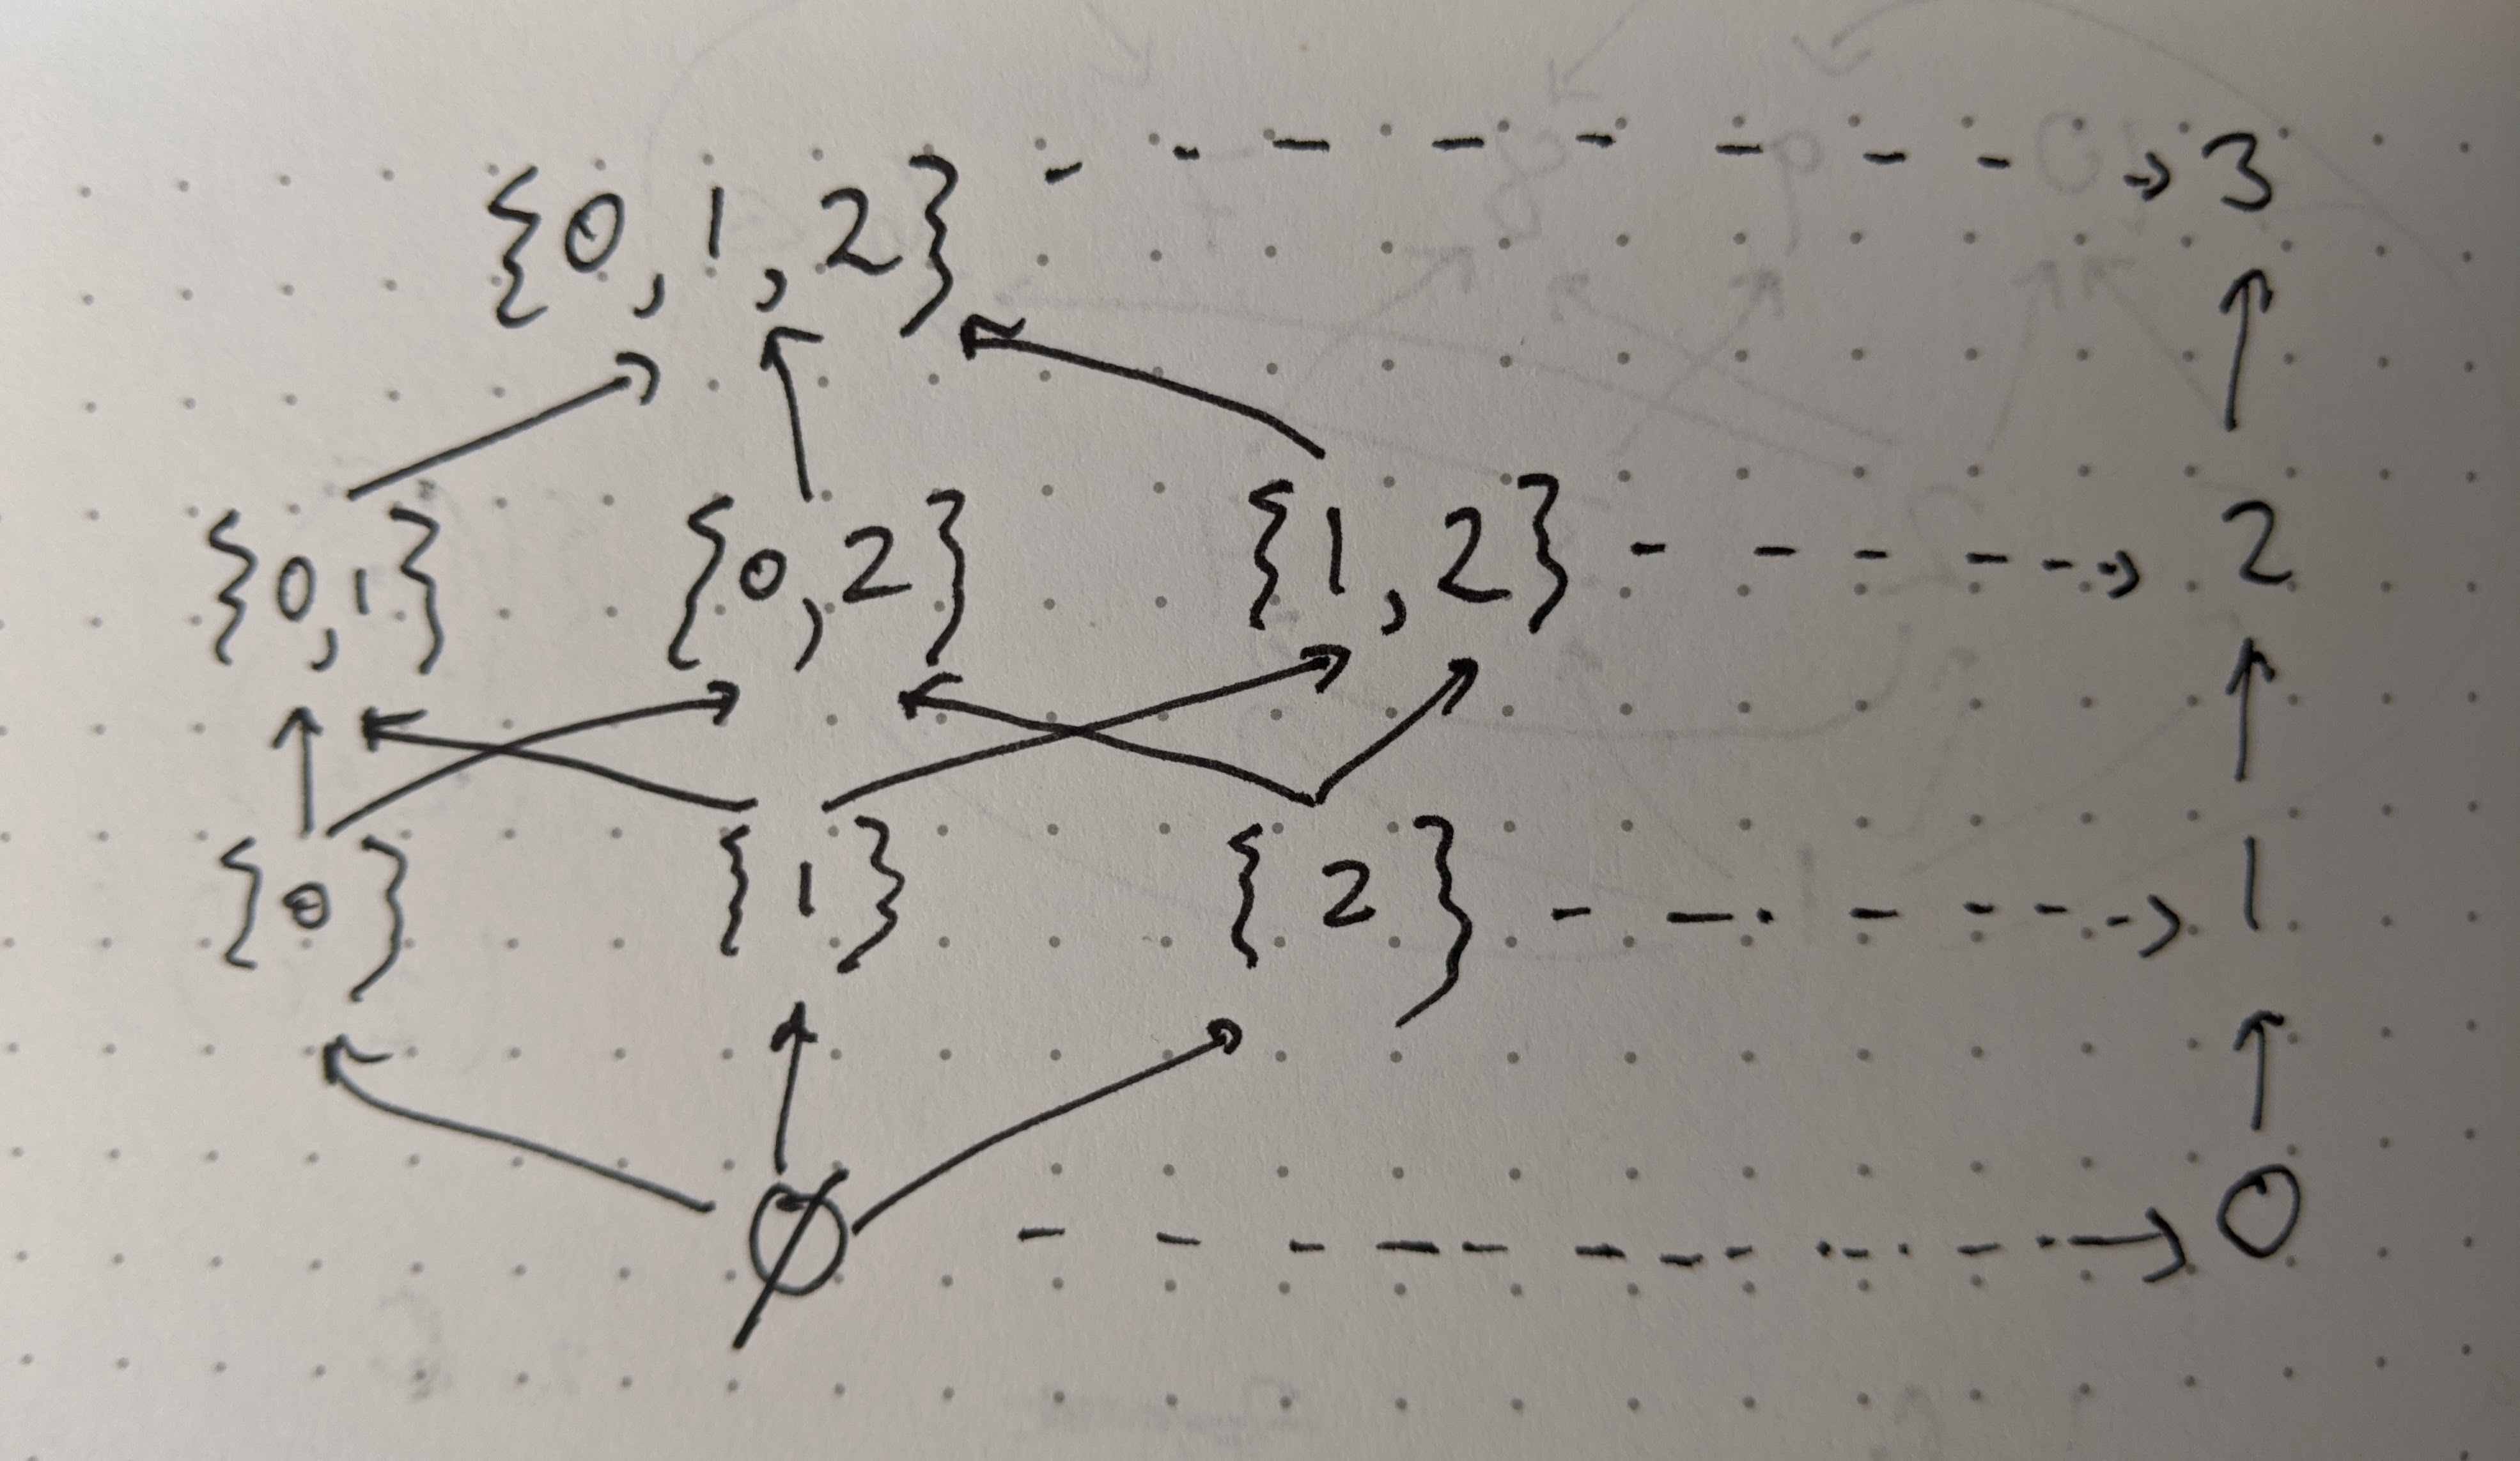
\includegraphics[width=0.5\linewidth]{images/1-63.jpg}

\exercise{1.65}
Draw the monotone map between $U(\B)$ and $P(\B)$ as described in the text.

\solution
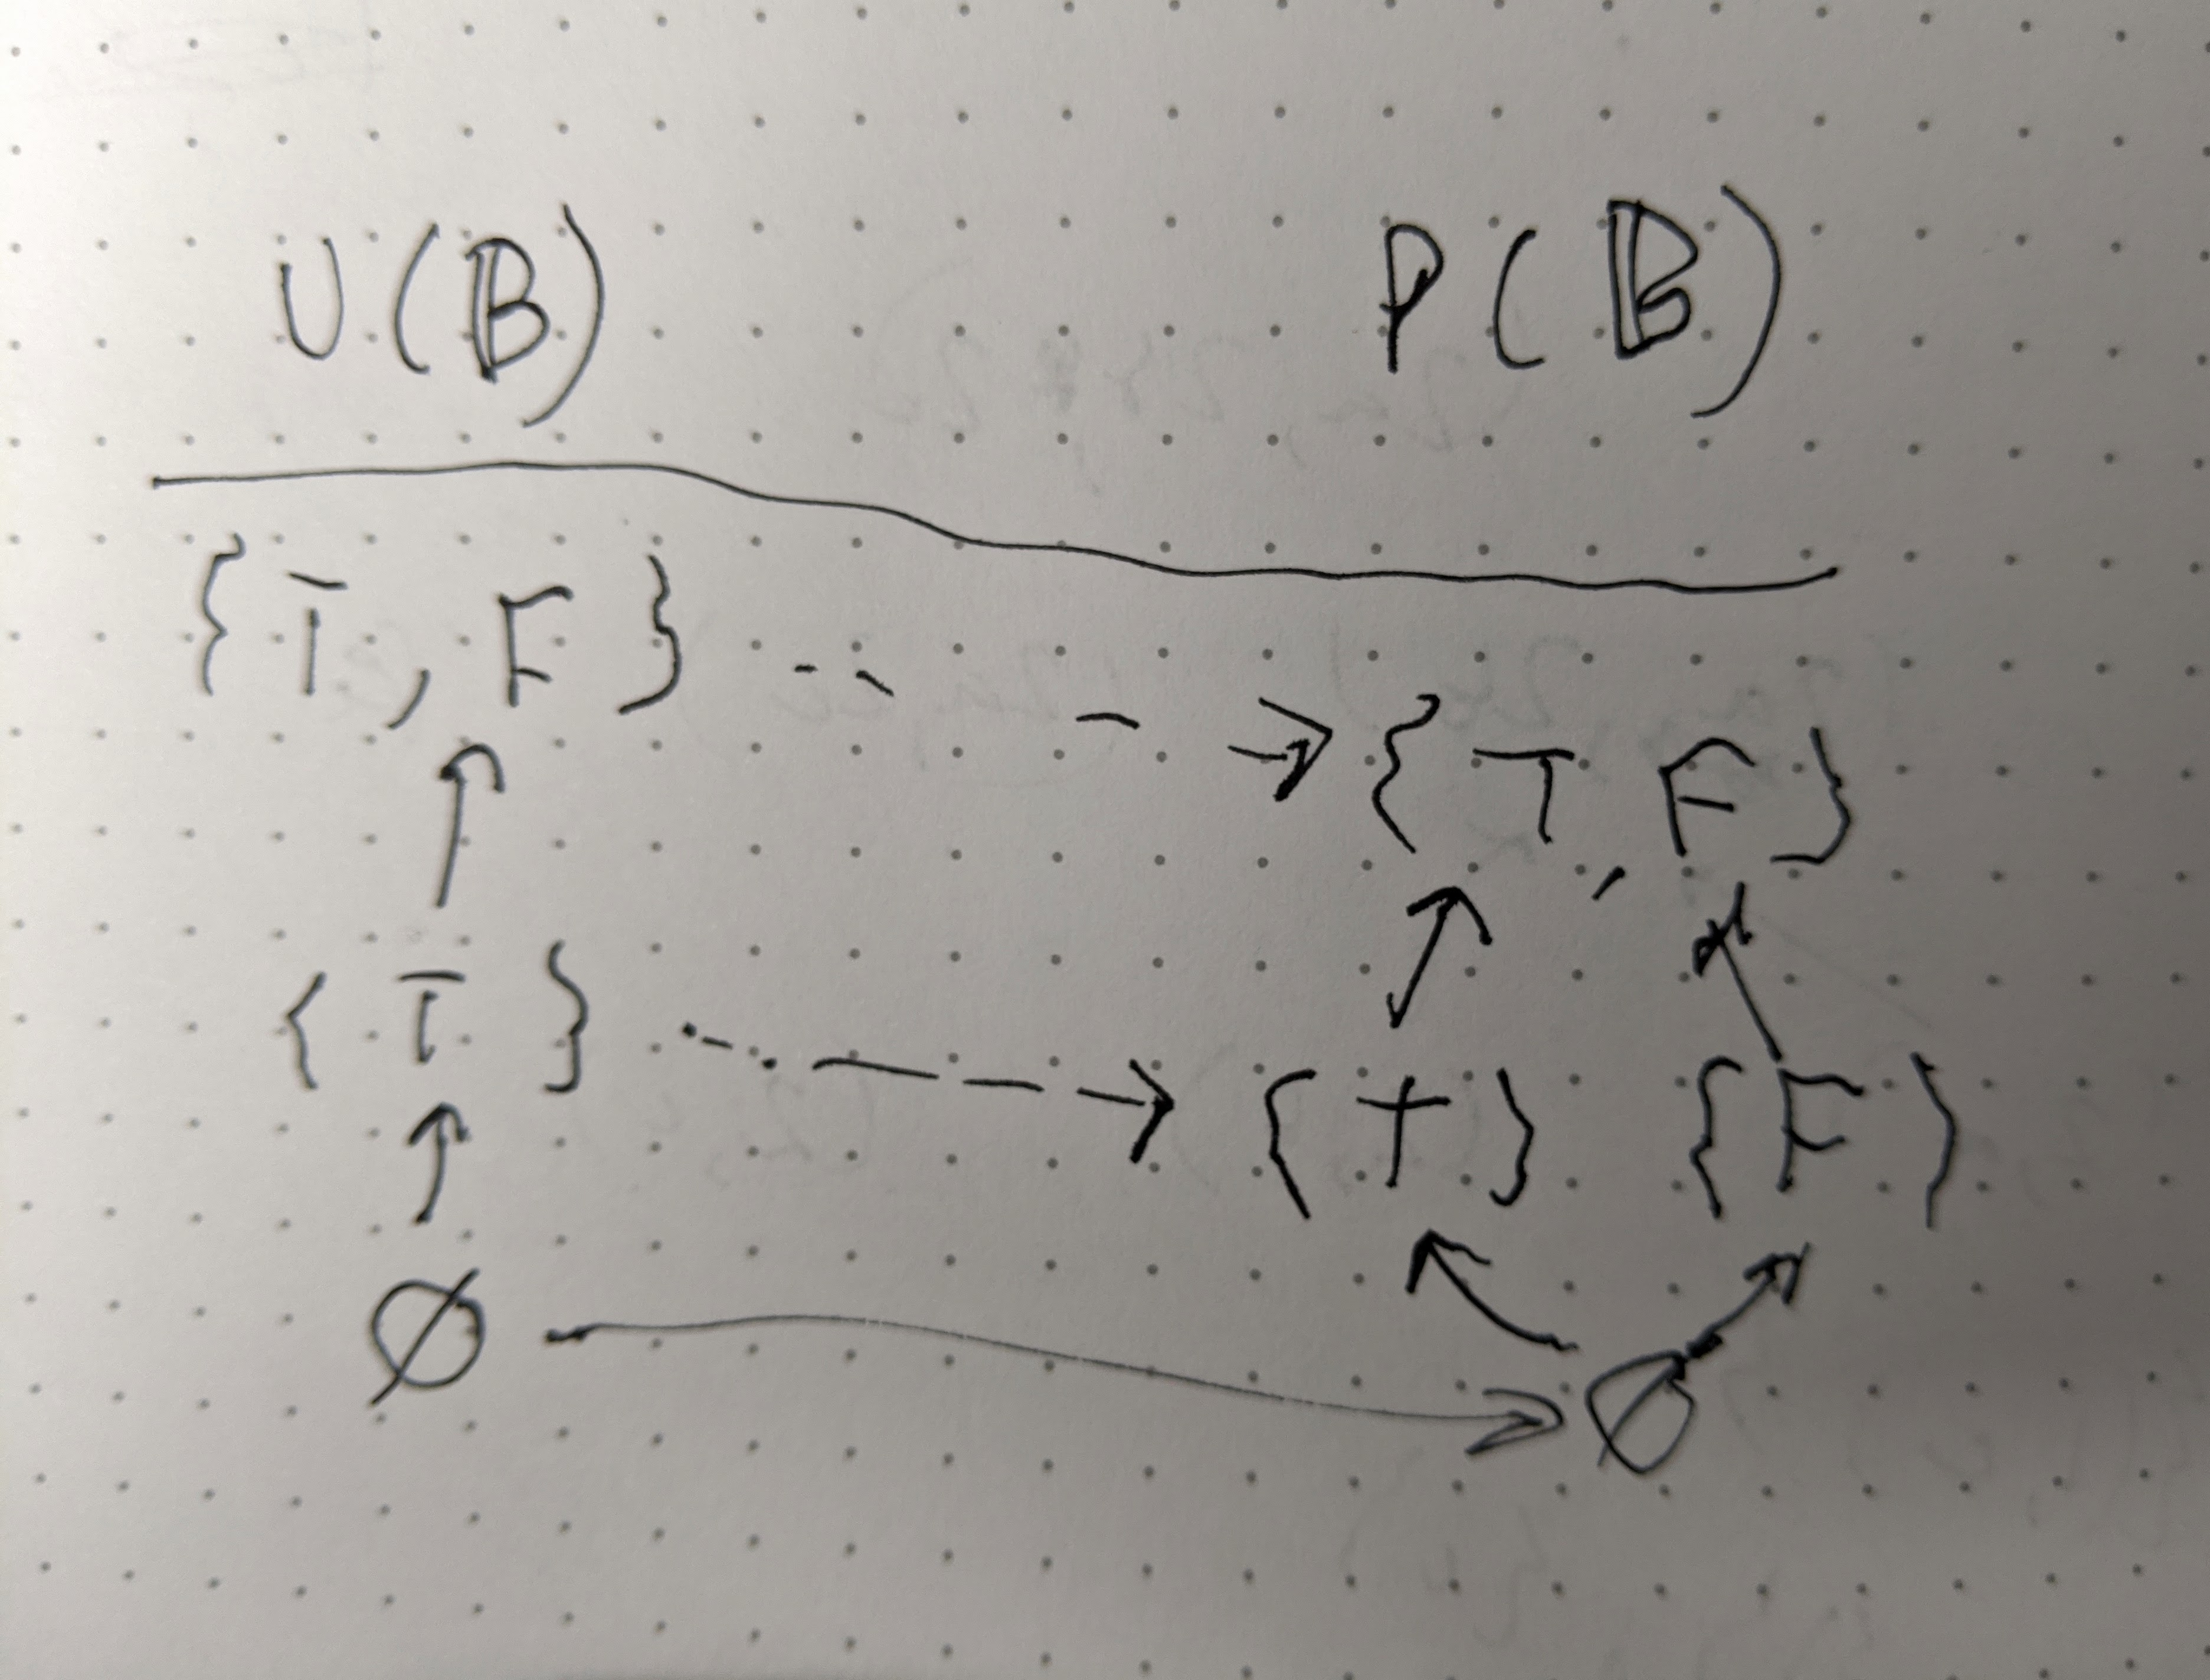
\includegraphics[width=0.5\linewidth]{images/1-65.jpg}

\exercise{1.66}
Let $(P, \leq)$ be a preorder.
\begin{enumerate}
    \item Show that the set $\uparrow p = \{p'\in P\ |\ p\leq p;\}$ is an upper set for any $p\in P$.
    \item Show that this defines a monotone map $\uparrow: P^{op}\to U(P)$.
    \item Show that $p\leq p'$ iff $\uparrow(p')\subseteq\uparrow(p)$.
    \item Draw a picture of the map $\uparrow$ in the case where $P$ is the preorder $(b\geq a\leq c)$.
\end{enumerate}

\solution
\begin{enumerate}
    \item Suppose $q\in \uparrow p$, then any $q'\geq q$ is transitively greater than $p$ and hence $q'\in \uparrow p$.
    \item Suppose $p\geq q$ (i.e. $p$ is less than $q$ in $P^{op}$), we want to show that $\uparrow p \subseteq \uparrow q$.  So let $p'\in \uparrow p$.  We know $q\leq p\leq p'$ and hence $p'\in\uparrow q$.
    \item We showed the first direction in part 2, so assume $\uparrow(p')\subseteq \uparrow(p)$.  This means $p\in \uparrow(p')$ and hence $p\leq p'$.
    \item 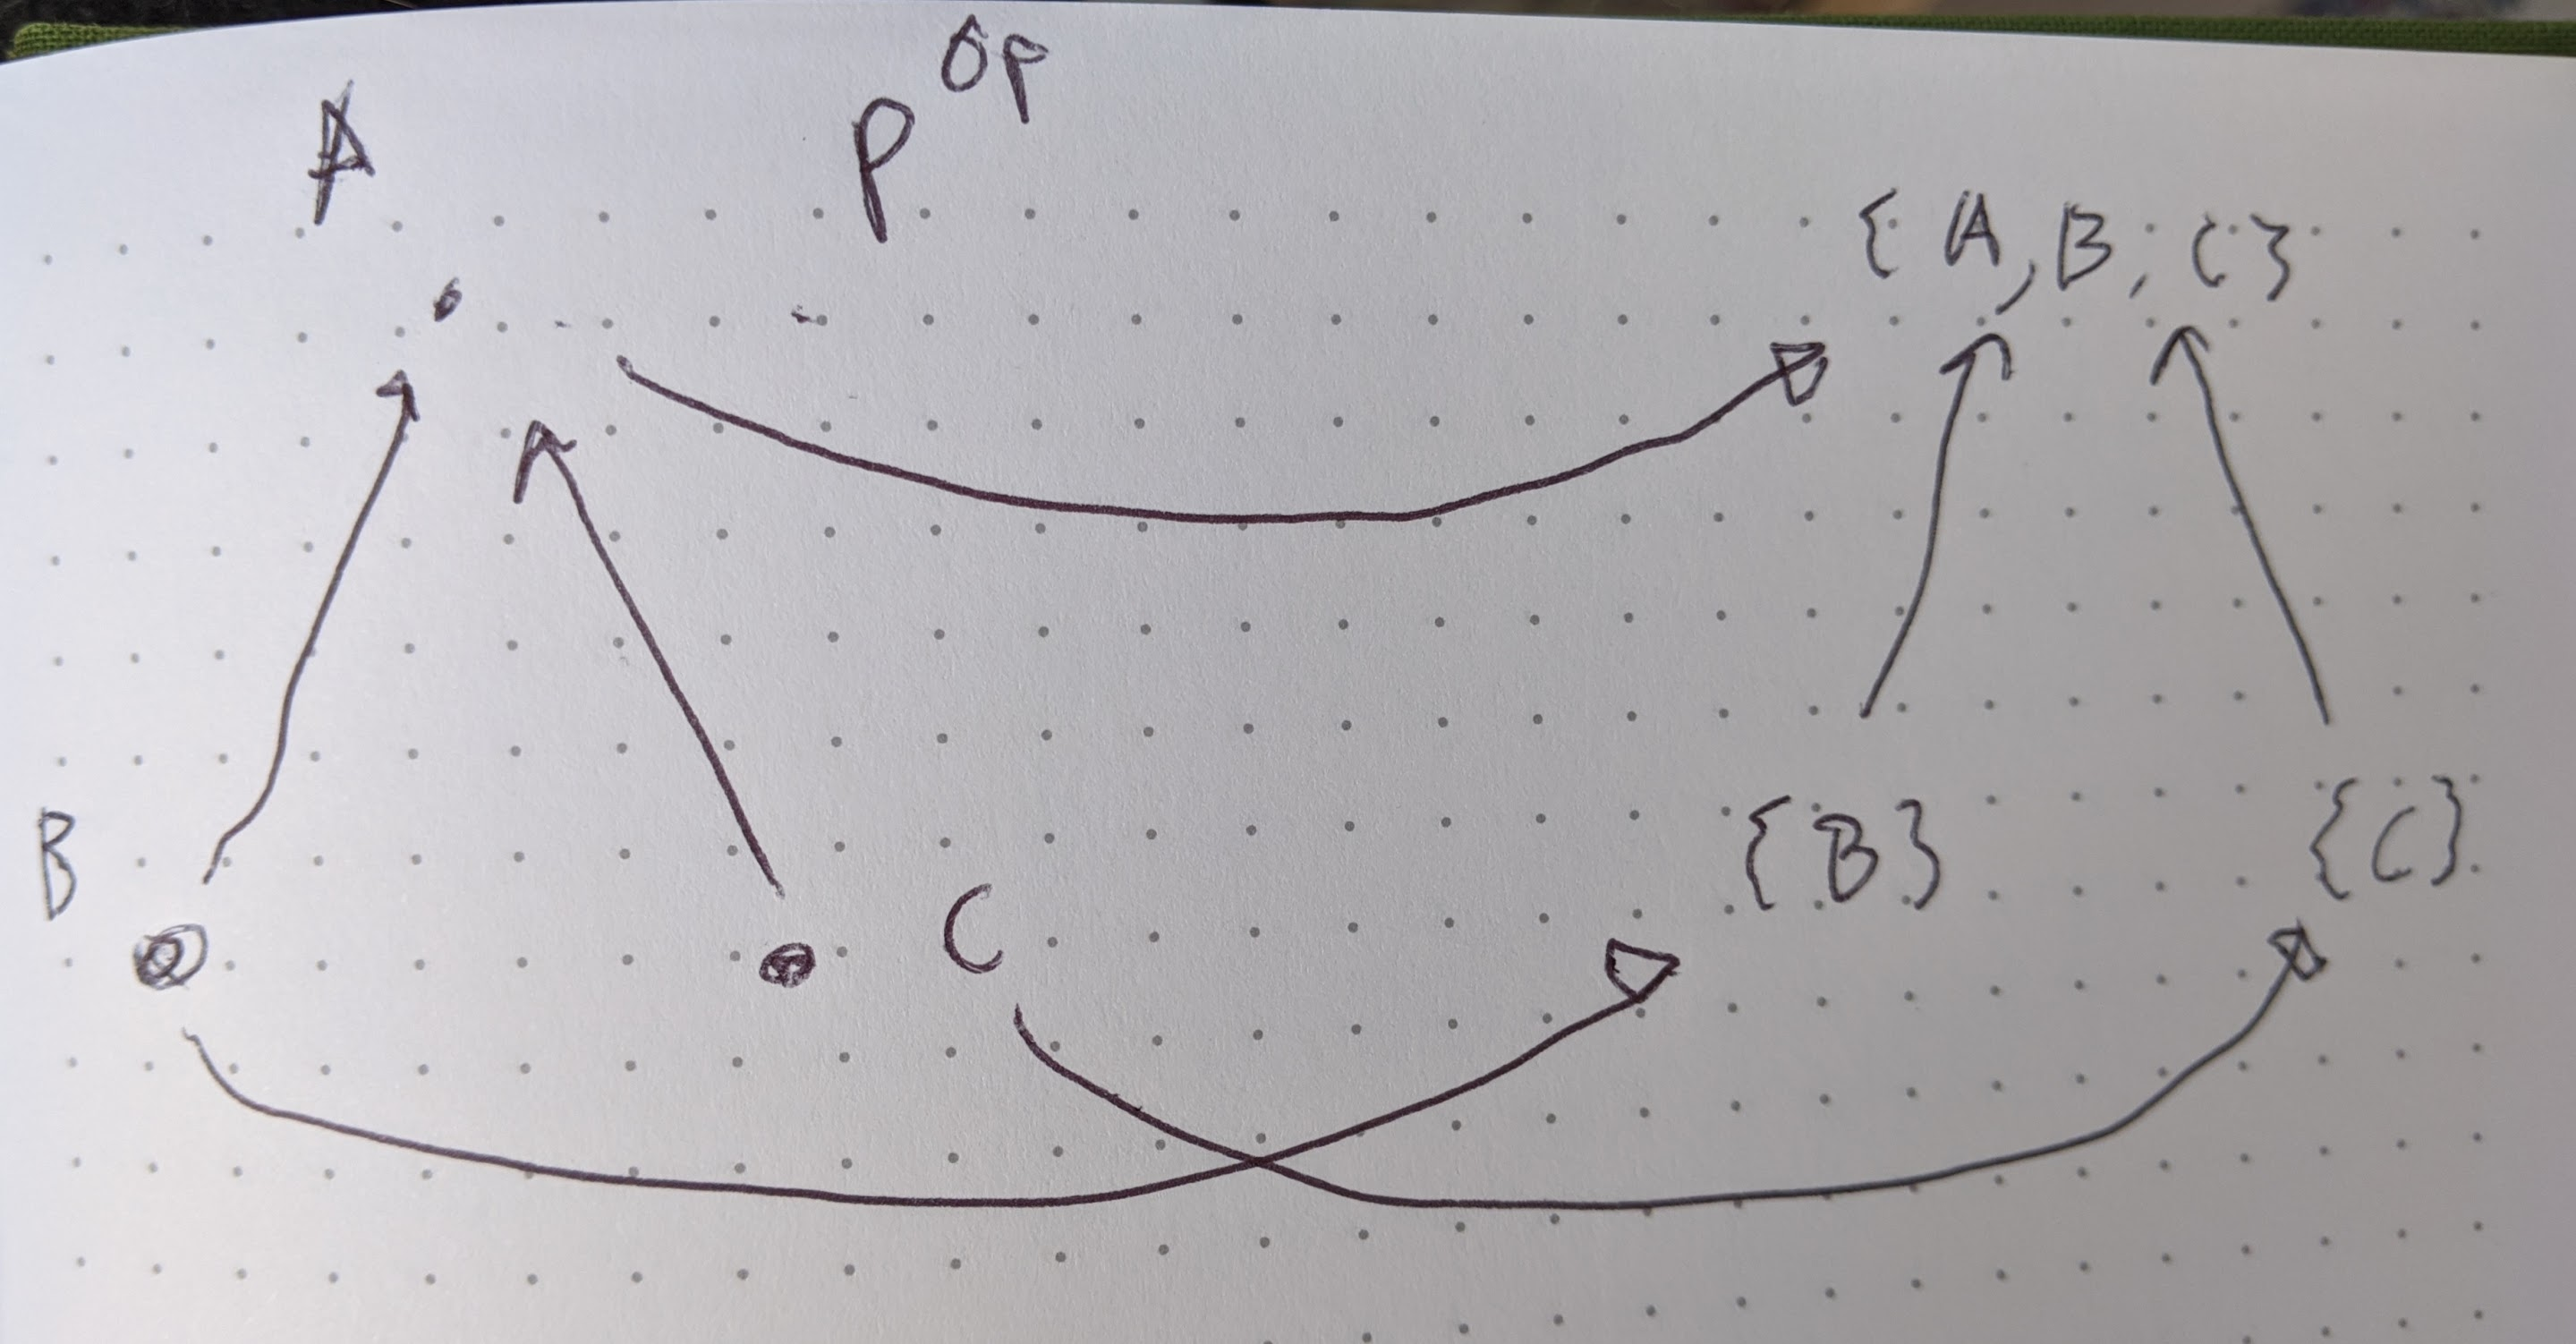
\includegraphics[width=0.5\textwidth]{images/1-66.jpg}
\end{enumerate}

\exercise{1.67}
Show that when $(P, \leq_P)$ is a discrete preorder, then every function $f:P\to Q$ is monotone regardless of the order $\leq_Q$.

\solution
We need to show that for any $x,y\in P$ where $x\leq_P y$, we have $f(x)\leq_Q f(y)$.  But the only $x$ and $y$ satisfying this are $x\leq_P x$, for which we have $f(x)\leq_Q f(x)$ regardless of $\leq_Q$ by the definition of a preorder.

\exercise{1.69}
Choose two sets $X$ and $Y$ with at least three elements each and choose a surjective, non-identity function $f:X\to Y$.  Write down two different partitions $P$ and $Q$ of $Y$, and find $f^*(P)$ and $f^*(Q)$.

\solution
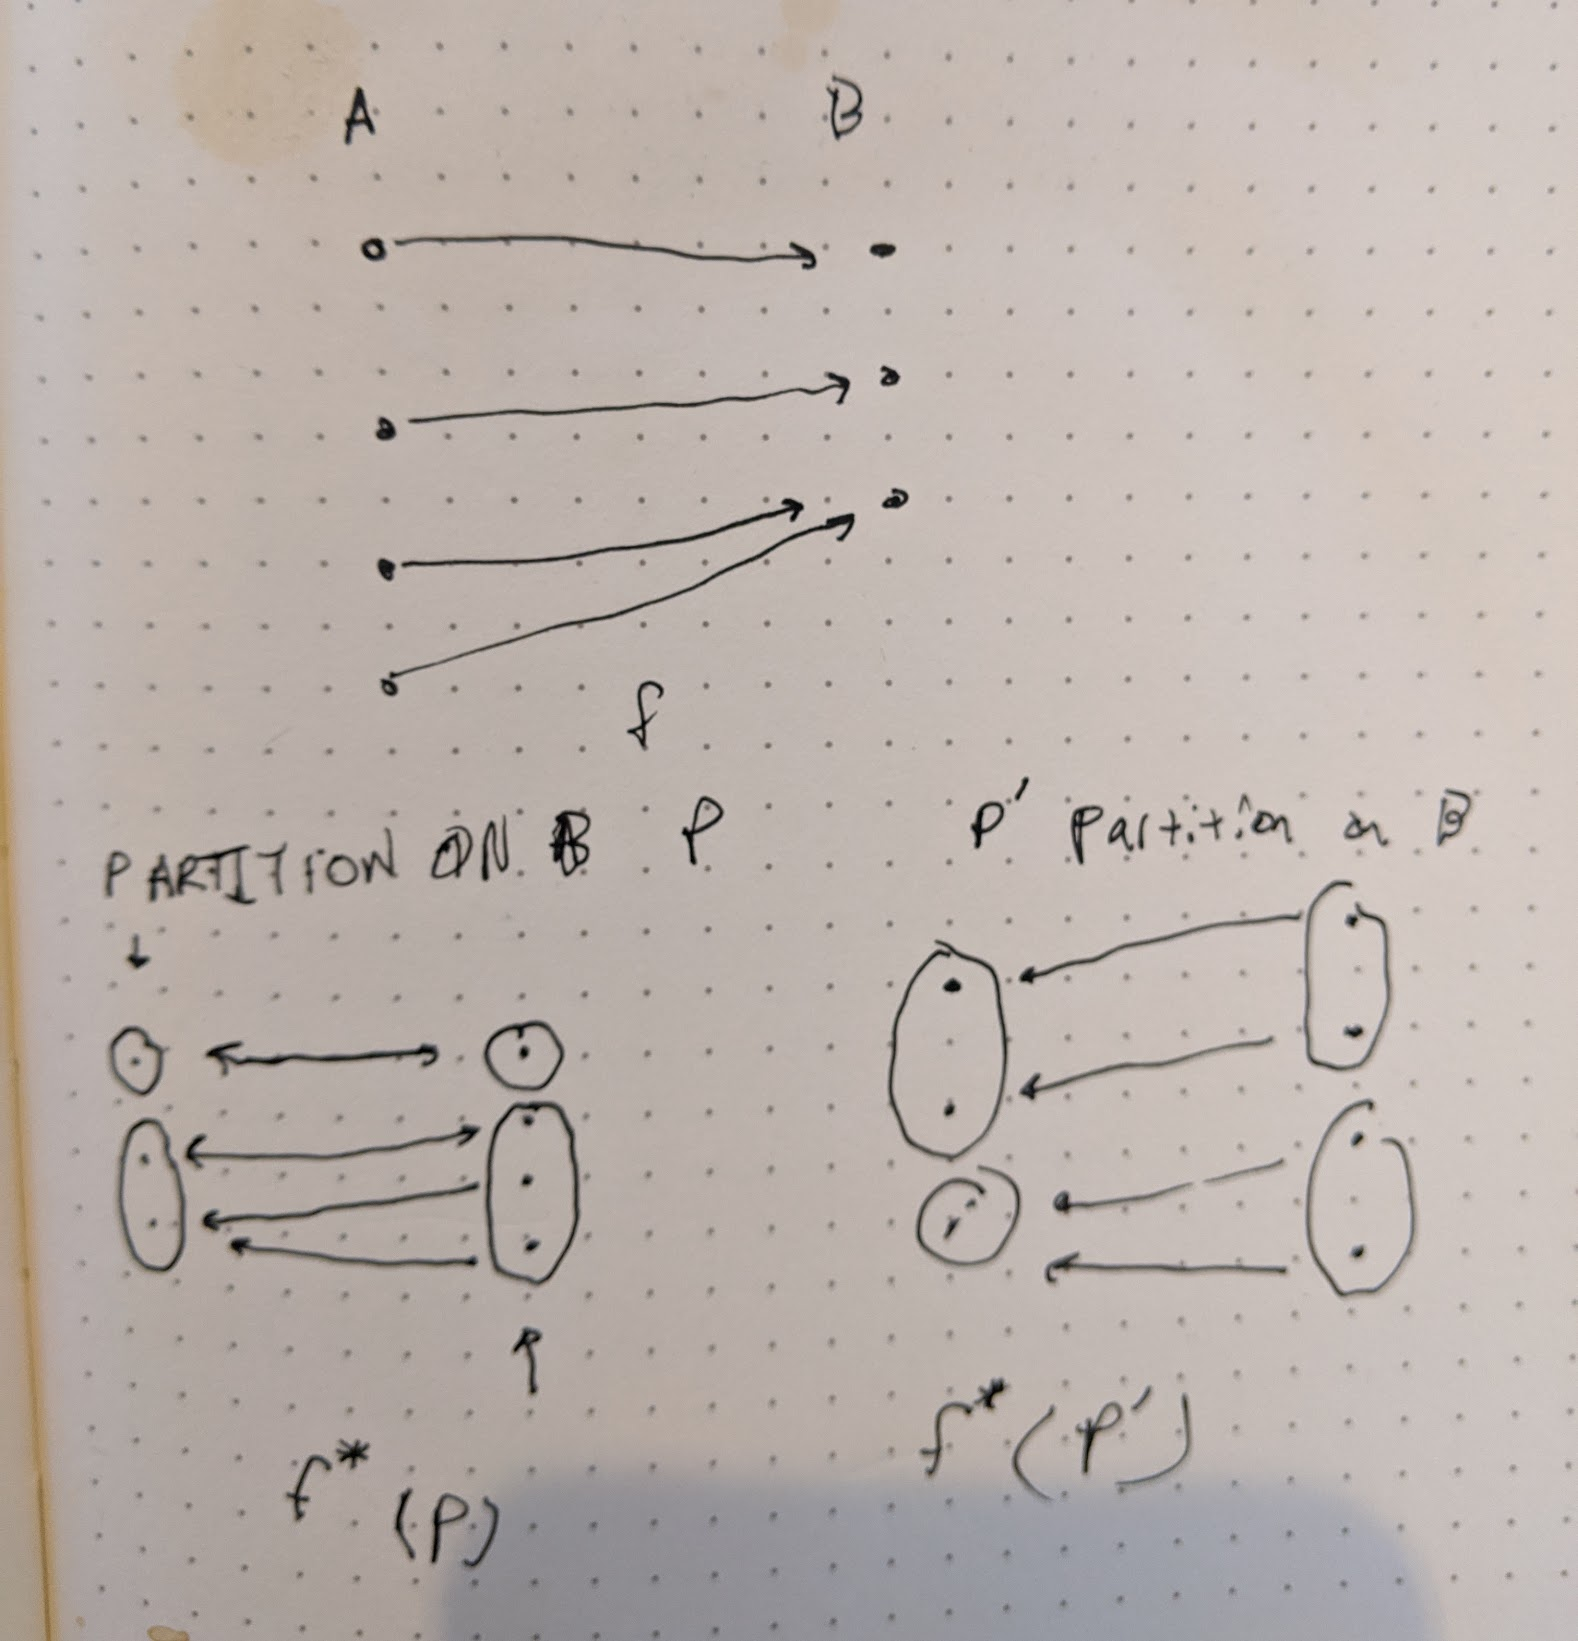
\includegraphics[width=0.5\linewidth]{images/1-69.jpg}

\exercise{1.71}
Prove Proposition 1.70:
\begin{enumerate}
    \item For any preorder $(P, \leq_P)$, the identity function is monotone.
    \item If $(Q, \leq_Q)$ and $(R, \leq_R)$ are preorders and $f:P\to Q$ and $g:Q\to R$ are monotone, then $(f\fcmp g):P\to R$ is also monotone.
\end{enumerate}

\solution
\begin{enumerate}
	\item If $a \leq_P b$ then clearly $a = f(a)\leq_P f(b) = b$ if $f$ is the identity function.
	\item Suppose $a\leq_P b$, then $f(a) \leq_Q f(b)$ as $f$ is monotone, and hence $g(f(a)) \leq_R g(f(b))$ as $g$ is also monotone.
\end{enumerate}

\exercise{1.73}
Show that a skeletal dagger preorder is just a discrete preorder, and hence can be identified with a set.

\solution
Let $(P, \leq)$ be a skeletal dagger preorder.  We need to show that for any $x\in P$, the only thing comparable to $x$ is $x$ itself.  So suppose $x\leq y$, then as $P$ is a dagger preorder we know that $y\leq x$.  Hence as $P$ is skeletal, we have that $x=y$.  This implies that $P$ is a discrete preorder.

\exercise{1.77}
Show that the map $\Phi$ from Section 1.1.1 (`Is $\bullet$ connected to $\star$?') is the monotone map $Prt(\{\star, \bullet, \circ\})\to\B$.

\solution
Let $P$ and $P'$ be partitions where $P\leq P'$.  If $\Phi(P)=\texttt{false}$ then clearly $\Phi(P)\leq\Phi(P')$, so assume $\Phi(P) = \texttt{true}$.  This means for some set $X$ in the partition $P$, we know that both $\bullet, \star\in X$.  As $P\leq P'$ this means there is some $Y$ in the partition $P'$  with $X\subseteq Y$, which implies that $\bullet,\star\in Y$.  Hence $\Phi(P')=\texttt{true}$ and $\Phi(P)\leq\Phi(P')$.

\exercise{1.79}
Let $P$ and $Q$ be preorders and $f:P\to Q$ a monotone map.  Show that the pullback $f^*:U(Q)\to U(P)$ can be defined by taking $u:Q\to\B$ to $(f\fcmp u):P\to\B$.

\solution
Call $\phi_Q$ the function that takes upper sets in $Q$ to monotone maps as defined in Proposition 1.78, and similarly $\phi_P$.  Let $U\in U(Q)$.  We want to show $\phi_P(f^{-1}(U)) = f\fcmp (\phi_Q(U))$.

Let $x\in P$.  If $x\in f^{-1}(U)$, then we know $\phi_P(f^{-1}(U))(x)=\texttt{true}$ by definition.  But we also know $f(x)\in U$ and hence $\phi_Q(U)(f(x)) = \texttt{true}$.  Conversely if $x\not\in f^{-1}(U)$, we will have both $\phi_P(f^{-1}(U))(x)=\texttt{false}$, as well as $f(x)\not\in U$ and $\phi_Q(U)(f(x)) = \texttt{false}$.  This shows that these maps are equal.

\exercise{1.80}
Why is 0 a greatest lower bound for $\left\{\frac{1}{n+1}\ |\ n\in\N\right\}\subseteq\R$?

\solution
Assume that $\varepsilon > 0$ is a lower bound. Let $n=\lceil 1 / \varepsilon \rceil$.  Then
\[
	\frac{1}{n+1}\leq \frac{1}{1 / \varepsilon +1} \leq \frac{1}{1/\varepsilon}=\varepsilon.
\]
Hence no such $\varepsilon$ is a lower bound.

\exercise{1.85}
Let $(P, \leq)$ be a preorder and $p\in P$, consider the set $A=\{p\}$.
\begin{enumerate}
	\item Show that $\bigwedge A \cong p$.
	\item Show that if $P$ is a partial order, then $\bigwedge A = p$.
	\item Are the analogous facts true when $\bigwedge$ is replaced by $\bigvee$?
\end{enumerate}

\solution
\begin{enumerate}
	\item Clearly $p\leq p$, so by definition $\bigwedge A \leq p$ (as a lower bound) and $\bigwedge A\geq p$ (as a greatest lower bound).
	\item If the previous is true in a partial order, then we have $\bigwedge A = p$.
	\item The analogous facts are true with $\bigvee$.
\end{enumerate}

\exercise{1.90}
In the $n|m$ ordering on $\N$, what are the meet and the join?

\solution
The meet is the greatest common divisor and the join is the least common multiple.

\exercise{1.94}
Prove that for any monotone map $f:P\to Q$, if $a, b\in P$ have a join and $f(a), f(b)\in Q$ have a join, then $f(a)\lor f(b)\leq f(a\lor b)$.

\solution
We know $a,b\leq a\lor b$, so since $f$ is monotone we have $f(a), f(b)\leq f(a\lor b)$.  Hence $f(a\lor b)$ is an upper bound for $\{f(a), f(b)\}$, so by definition of the join we must have $f(a)\lor f(b)\leq f(a\lor b)$.

\exercise{1.98}
Find a right adjoint for the monotone map $(3\times -):\Z\to\R$, and show it is correct.

\solution
Let $g(y) = \lfloor y/3 \rfloor$.  Then we have $3x \leq y \iff x\leq y/3 \iff x\leq \lfloor y/3\rfloor$, hence $g$ is a right adjoint for $3x$.

\exercise{1.99}
See book.

\solution
\begin{enumerate}
	\item In this case $f$ is left adjoint to $g$.
	\item In this case $f$ is not left adjoint to $g$, as $g(1)=2\geq 2$ but $f(2)=2\nleq 1$.
\end{enumerate}

\exercise{1.101}
\begin{enumerate}
	\item Does $\lceil -/3\rceil$ have a left adjoint $L:\Z\to\R$?
	\item If not, why?  If so, does its left adjoint have a left adjoint?
\end{enumerate}

\solution
Let $g:\R\to\Z$ be defined by $g(x)=\lceil x/3 \rceil$.  We will show by contradiction that $g$ does not have a left adjoint.

For a left adjoint $f:\Z\to\R$, we must have $f(1)\leq 0 \iff 1\leq g(0)=\lceil 0/3\rceil=0$.  Clearly the second part does not hold, so we know $f(1)\nleq 0$.

On the other hand, we know that $f(1)\leq \inf A$ where $A=\{x | g(x)\geq 1, x\in\R\}$.  However $1/n\in A$ for $n\in\Z^+$, as $\lceil 1/n\rceil = 1$ for all such $n$.  But $\inf\{1/n | n\in\Z^+\}=0$, which implies that $f(1)\leq 0$.  This is a contradiction, so $g$ must not have a left adjoint.

\exercise{1.103}
Choose 6 different partitions on the set $S$ and for each, call it $c$, find $g_!(c)$ where $S, T,$ and $g:S\to T$ are the same as they were in Example 1.102.

\exercise{1.105}
Using the same $S, T,$ and $g:S\to T$ as in Example 1.102, find the partition $g^*(c)$ for each of the 5 partitions $c$ on the set $T$.

\solution
For both 1.103 and 1.105.

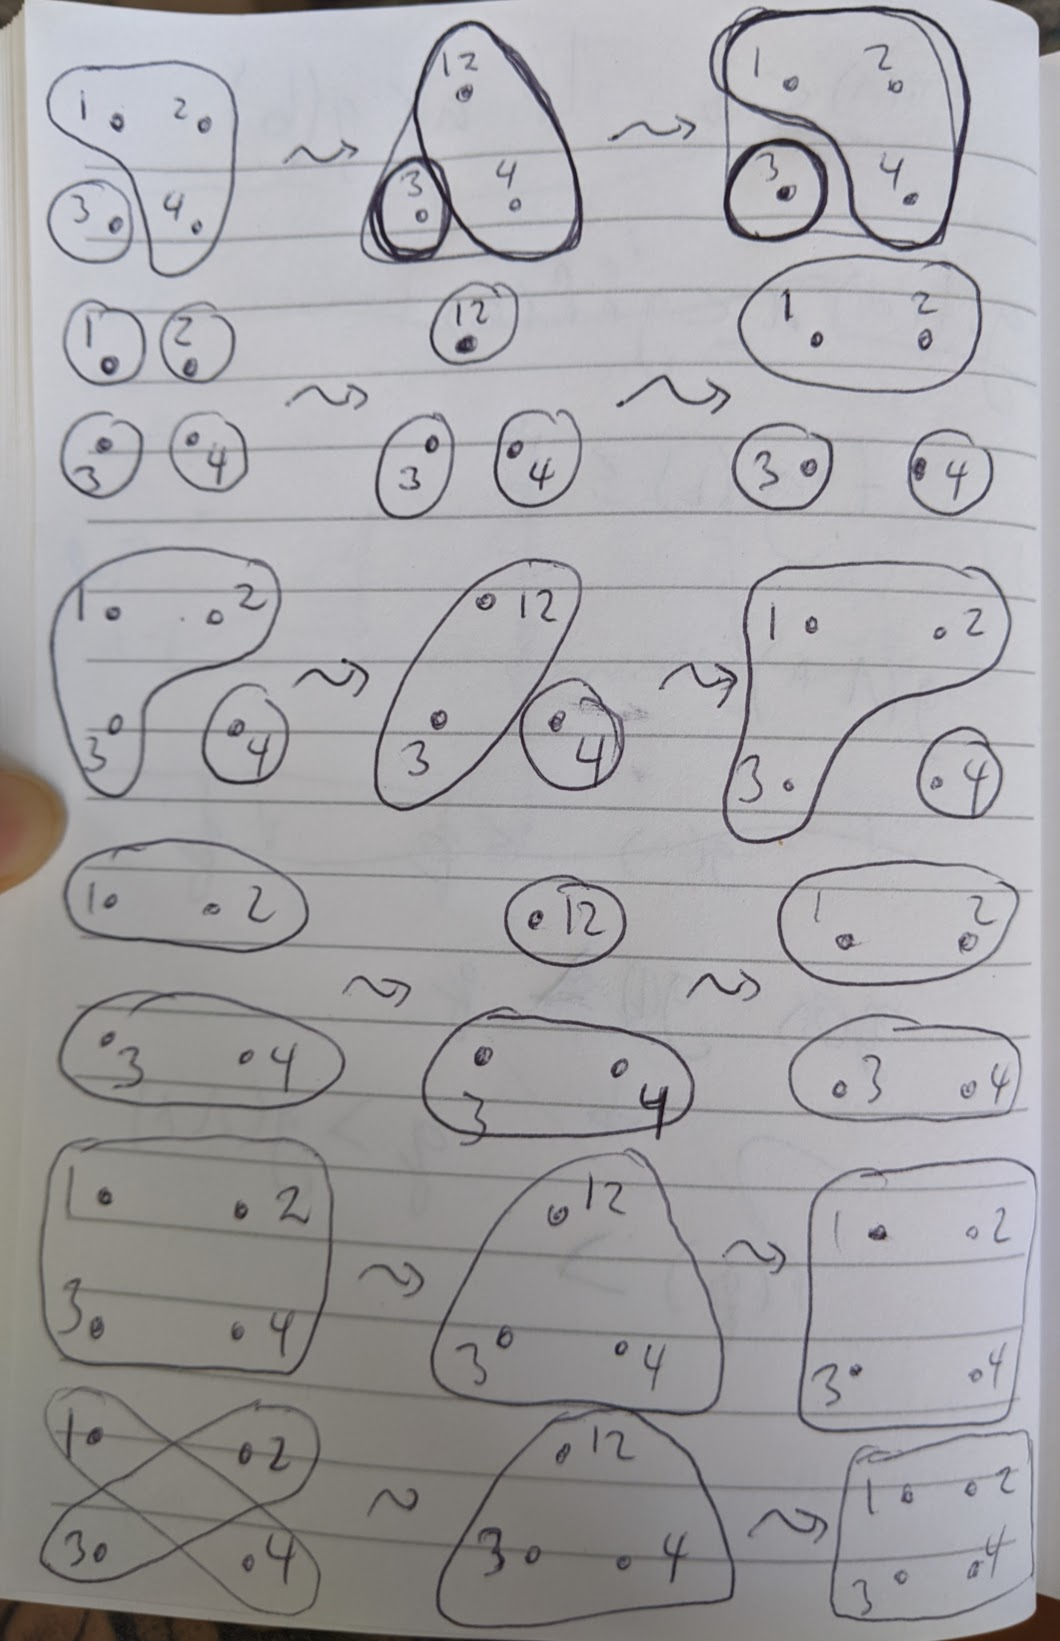
\includegraphics[width=0.5\linewidth]{images/1-105.jpg}

\exercise{1.106 (revised)}
Prove that $g_!$ is left adjoint to $g^*$, as defined in the text.
%Let $S,T,$ and $g:S\to T$ be as in Example 1.102.
%\begin{enumerate}
%	\item Choose a nontrivial partition $c:S\to P$ and let $g_!(c)$ be its push forwards partition on $T$.
%	\item Choose any coarser partition $d:T\to P'$, i.e. where $g_!(c)\leq d$.
%	\item Choose any non-coarser partition $e:T\to Q$, i.e. where $g_!(c)\nleq e$.
%	\item Find $g^*(d)$ and $g^*(e)$.
%	\item Since $g_!(c)\leq d$ and $g_!(c)\nleq e$, we should have $c\leq g^*(d)$ and $c\nleq g^*(e)$.  Show that this is true.
%\end{enumerate}

\solution

Let $S, T$ be sets, and let $g: S \to T$.  Define $g_{!}, g^{*}$ as in the text.  

We first show $g^{*}$ is monotone.  Let $A, B\in Prt(T)$ such that $A\leq B$.  Then for each set $A_i\in A$, $A_i \subseteq B_j$ for some $B_j\in B$, and as a result $g^{-1}(A_i)\subseteq g^{-1}(B_j)$ for each $A_i\in A$.  As the image of a partition under $g^*$ is the collection of preimages of that partition via $g$, we have $g^{*}(A)\leq g^{*}(B)$.

Next we show $g_!$ is monotone.  Let $A, B\in Prt(S)$ such that $A\leq B$.  As before we know that for each set $A_i\in A$, $A_i\subseteq B_j$ for some $B_j\in B$. We consider $A,B\in Rel(S)$ i.e. subsets of $S\times S$. Note that $g_{!}(C)$  is the transitive closure of the relation $\{ (g(x),g(y)| (x, y)\in C\}$.  As $A\leq B$, $\{ (g(x),g(y)| (x, y)\in A\}\subseteq \{ (g(x),g(y)| (x, y)\in B\}$.  Using the fact that the function taking a relation to its transitive closure is monotone on the set of relations ordered by inclusion, we can conclude that $g_{!}(A)\leq g_{!}(B)$.

For the next part of the proof, we use proposition 1.107, and  derive our result by showing that for each $A\in Prt(S)$ and for each $B\in Prt(T)$ that both $A\leq g^*\circ g_!(A)$, and $g_!\circ g^*(B)\leq B$. 

 We start with showing $A\leq g^*\circ g_!(A)$. First we consider two additional functions, first $\bar{g}: Prt(S) \to Rel(T)$, where $g(r) = \{(g(x),g(y))| (x,y)\in r\}$.  Secondly an extension of $g^*$ to all relations, $\bar{g^*}:Rel(T)\to Rel(S)$, so for a relation $r$, we have $\bar{g^*}(r) = \{(x,y)| (g(x),g(y))\in r\}$ ($g^*$ is the restriction of $\bar{g^*}$ to equivalence relations).  Both $\bar{g}$ and $\bar{g^*}$ are monotone, which can be seen in proofs similar to our proofs for $g^*$ and $g_!$.  Additionally let the transitive closure of a set $Q$ be denoted $\hat{Q}$. We now note two things, one $A = \bar{g^*}\circ \bar{g}(A)$, and two $ g^*\circ g_!(A) = \bar{g^*}( \widehat{\bar{g}(A)})$.  As $\bar{g^*}$ is monotone and $\bar{g}(A)\leq \widehat{\bar{g}(A)}$ we have $A\leq g^*\circ g_!(A)$.
 
 % TODO

\exercise{1.109}
Complete the proof of Proposition 1.107 by showing that (for monotone $f:P\to Q$ and $g:Q\to P$)
\begin{enumerate}
	\item if $f$ is left adjoint to $g$ then for any $q\in Q$ we have $f(g(q))\leq q$, and
	\item if $p\leq g(f(p))$ and $f(g(q))\leq q$, then $p\leq g(p)$ iff $f(p)\leq q$ holds, for all $p\in P$ and $q\in Q$.
\end{enumerate}

\solution
Assume $f$ is left adjoint to $g$.  Let $q\in Q$ and $p=g(q)$. Then we know $p\leq g(q)$, so by definition of the left adjoint $f(p)\leq q$.  As we defined $p$ to be $g(q)$ this implies $f(g(q))\leq q$.

Next assume $p\leq g(f(p))$ and $f(g(q))\leq q$ for any $p\in P, q\in Q$.  We need to show that $p\leq g(q)$ implies $f(p)\leq q$.  But $p\leq g(q)$ implies $f(p)\leq f(g(q))$ by the monotonicity of $f$, and $f(g(q))\leq q$ by assumption, so $f(p)\leq q$.

\exercise{1.110}
\begin{enumerate}
	\item Show that if $f:P\to Q$ has a right adjoint $g$, then it is unique up to isomorphism.  That is, for any other right adjoint $g'$, we have $g(q)\cong g'(q)$ for all $q\in Q$.
	\item Is the same true for left adjoints?  That is, if $h:P\to Q$ has a left adjoint, is it necessarily unique up to isomorphism?
\end{enumerate}

\solution
\begin{enumerate}
\item Suppose $g$ and $g'$ are right adjoint to $f:P\to Q$.  Then for any $q\in Q, p\in P$ we have
$$f(p)\leq q\iff p\leq g(q)\iff p\leq g'(q).$$
In particular this holds for $p=g(q)$, which means $g(q)\leq g'(q)$ as by reflexivity $g(q)\leq g(q)$.  Similarly for $p=g'(q)$, we have $g'(q)\leq g(q)$ as $g'(q)\leq g'(q)$.  Thus $g(q)\cong g'(q)$ for all $q\in Q$.

\item The same holds for left adjoints.  To show this, suppose $f$ and $f'$ are left adjoint to $g:Q\to P$.  Then for any $p\in P,q\in Q$ we have
$$f(p)\leq q\iff p\leq g(q)\iff f'(p)\leq q.$$
The rest of the proof follows analogously to part 1.
\end{enumerate}

\exercise{1.112}
Complete the proof of Proposition 1.111 by showing that left adjoints preserve joins.

\solution





\chapter{Resource Theories}

\exercise{2.5}
Is $(\R, \leq, 1, *)$ a symmetric monoidal preorder?

\solution
It is not a monoidal preorder, as for example $-5\leq -1$ and $-2\leq -1$, but $-5*-2\nleq -1*-1$.

\exercise{2.8}
Check that if $(M, *,e)$ is a commutative monoid then $(\textbf{Disc}_M,=,*,e)$ is a symmetric monoidal preorder.

\solution
Unitality, associativity, and symmetry come for free from the definition of a commutative monoid, so we only need to check monotonicity.  Since $x\leq y\iff x=y$ this is easy to check, as $x_1\leq y_1$ and $x_2\leq y_2$ implies $x_1=y_1$ and $x_2=y_2$ which in turn implies that $x_1*x_2 = y_1 * y_2$.

\newpage

\exercise{2.20}
Formally prove that $t\leq v+w, w+u\leq x+z, v+x\leq y$ implies $t+u\leq y+z$.  Be explicit about where reflexivity and transitivity are used, and why symmetry need not be used.

\solution
In the below, R=reflexivity, M=monotonicity, A=associativity, T=transitivity.  Symmetry is not used, which you can tell from the diagram from the fact that no wires cross.
\begin{align}
	t\leq v+w, u\leq u &&\implies&& t+u\leq (v+w)+u = v+(w+u) &\quad& \textrm{[R, M, A, T]}\label{1} \\
	(\ref{1}),w+u\leq x+z &&\implies&& v+(w+u)\leq v+(x+z) &\quad& \textrm{[M]}\label{2} \\
	(\ref{1},\ref{2}) &&\implies&& t+u\leq v+(x+z) = (v+x)+z &\quad& \textrm{[T, A]}\label{3} \\
	v+x\leq y, z\leq z &&\implies&& (v+x)+z\leq y+z &\quad& \textrm{[M]}\label{4} \\
	(\ref{3},\ref{4}) &&\implies&& t+u\leq y+z &\quad& \textrm{[T]}\label{5}
\end{align}

\exercise{2.21}
Skipped.

\exercise{2.29}
Consider $(\B,\leq)$ with monoidal product $\lor$.  What's the monoidal unit?  Does it satisfy the rest of the conditions?

\solution
The monoidal unit should be $\texttt{false}$.  Discussed why in person (i.e. truth table)

\exercise{2.31}
Show that there is a monoidal structure on $(\N, \leq)$ where the monoidal product is standard $*$.  What should the monoidal unit be?

\solution
The monoidal unit should be 1.  We will show monotonicity as the other conditions are obvious.  If $x_1\leq y_1$ and $x_2\leq y_2$, then there are $a_1,a_2\in\N$ such that $y_1 = x_1+a_1$ and $y_2=x_2+a_2$.  Then
$$y_1 * y_2 = (x_1 + a_1) * (x_2 + a_2)= x_1*x_2+a_1*x_2 + a_2*x_1 + a_1*a_2\geq x_1*x_2.$$

\exercise{2.33}
Consider the divisibility order $(\N, |)$.  Does $0$ as monoidal unit and $+$ as monoidal product satisfy the conditions?

\solution
It does not, as for example $2|4$ and $1|1$, but $(2+1)\nmid(4+1)$, so monotonicity fails.

\exercise{2.34}
Consider the preorder $\textbf{NMY}$ with Hasse diagram $\texttt{no}\to\texttt{maybe}\to\texttt{yes}$, monoidal unit $\texttt{yes}$ and ``min'' as the monoidal product.  Define what ``min'' should be and check that the axioms hold.

\solution
\begin{tabular}{c|ccc} 
min & no & maybe & yes \\
\hline no & no & no & no \\
maybe & no & no & maybe \\
yes & no & maybe & yes
\end{tabular}

\exercise{2.35}
Let $S$ be a set and let $P(S)$ be its power set, with the subset relation as order.  Does $P(S)$ with unit $S$ and product given by set intersection satisfy the conditions of symmetric monoidal preorder?

\solution
The other conditions are easy to show, so we will show monotonicity only.  Let $A_1, A_2, B_1, B_2\subseteq S$ where $A_1\subseteq B_1$ and $A_2\subseteq B_2$.  Then $A_1\cap A_2 \subseteq A_1\subseteq B_1$ and $A_1\cap A_2\subseteq A_2\subseteq B_2$, which implies that $A_1\cap A_2\subseteq B_1\cap B_2$.

\exercise{2.36}
Let $\texttt{Prop}^\N$ denote the set of all mathematical statements one can make about a natural number, where we consider two statements to be the same if one is true if and only if the other is true.  Given $P,Q\in\texttt{Prop}^\N$, we say $P\leq Q$ if for all $n\in\N$, whenever $P(n)$ is true, so is $Q(n)$.  Define a monoidal unit and product on $\texttt{Prop}^\N$.

\solution
We define the monoidal unit to be the statement ``$n$ is a natural number'' (i.e. a statement that's always true) and the monoidal product to be logical AND.  Note that this SMP effectively reduces to the previous example, where we consider subsets $P = \{n\in\N\ | P(n)\}$.

\exercise{2.39}
Complete the proof of Proposition 2.38.

\solution
These conditions are inherited from the original SMP, so we have decided this problem is dumb.

\exercise{2.40}
What is $\textbf{Cost}^\textrm{op}$ as a preorder?  What is the monoidal unit and product?

\solution
$\textbf{Cost}^\textrm{op}$ is the same as $\textbf{Cost}$ but using $\leq$ rather than $\geq$.  From Proposition 2.38, we know that $\textbf{Cost}^\textrm{op}$ can use the same monoidal unit and product as the original, i.e. $0$ and $+$.

\exercise{2.43}
Check that the map $g:(\B, \leq, \true, \land)\to([0,\infty],\geq,0,+)$ with $g(\false) = \infty$ and $g(\true)=0$ is monoidal monotone.  Is $g$ strict?

\solution
Clearly $g(\false)\leq g(\true)$ as $\infty\geq 0$, so $g$ is monotone.  In addition $g(\true)=0$, so the function preserves identities exactly.  Finally note that $g(\false)+g(\false) = \infty + \infty = \infty = g(\false)=g(\false\land\false)$, the other products are trivial as we've shown the identity is preserved.  Hence $g$ is strict monoidal monotone.

\exercise{2.44}
Let $\textbf{Bool}$ and $\textbf{Cost}$ be as above, and consider $d,u:[0,\infty]\to\B$ as follows:
$$d(x):=\left\{\begin{array}{ll}\text { false } & \text { if } x>0 \\ \text { true } & \text { if } x=0\end{array} \quad\quad\quad u(x):=\left\{\begin{array}{ll}\text { false } & \text { if } x=\infty \\ \text { true } & \text { if } x<\infty\end{array}\right.\right.$$
Is $d$ monotonic, monoidal, and/or strict?  Is $u$?

\solution

\exercise{2.45}
\begin{enumerate}
	\item Is $(\N, \leq, 1, *)$ a monoidal preorder?
	\item If not, why not?  If so, does there exist a monoidal monotone $(\N,\leq, 0, +)\to (\N, \leq, 1,*)$?  If not, why not?
	\item Is $(\Z,\leq, *, 1)$ a monoidal preorder?
\end{enumerate}

\solution



\chapter{Databases}

\exercise{3.3}
Discussed in person.

\exercise{3.9}
Check that $\Free(G)$ is a category for any graph $G$.

\solution
It is clear that concatenating any path with the trivial path yields the original, so unitality is satisfied.  Concatenation of paths is also associative (you can think of paths as lists of vertices/edges, which makes this clear).

\exercise{3.10}
Discussed in person

\exercise{3.12}
\begin{enumerate}
	\item What is the category $\textbf{1}$?
	\item What is the category $\textbf{0}$?
	\item What is the formula for the number of morphisms in $\textbf{n}$ for arbitrary $n\in\N$?
\end{enumerate}

\solution
\begin{enumerate}
	\item $\textbf{1}$ has a single object and only the identity morphism; it corresponds to the free category on the graph with one vertex.
	\item $\textbf{0}$ has no objects and no morphisms.
	\item The number of morphisms is $\sum_{i=1}^n i = \frac{n(n+1)}{2}$.  This is because there is one path of length $n-1$, two of length $n-2$, and so on until you get $n$ paths of length 1.
\end{enumerate}

\exercise{3.15}
In the loop graph, we identified paths with numbers $n\in\N$.  Given $m,n\in\N$, what number corresponds to the concatenation of their associated paths?

\solution
The concatenation corresponds to $m+n$.

\exercise{3.16}
\begin{enumerate}
	\item Write down the 10 paths in the free square category.
	\item Name two distinct parallel paths.
	\item Name two paths that are not parallel.
\end{enumerate}

\solution
\begin{enumerate}
	\item $\id_A, \id_B, \id_C, \id_D, f, g, h, i, f\fcmp h, g\fcmp i$
	\item $f\fcmp h$ and $g\fcmp i$
	\item $f$ and $g$
\end{enumerate}

\exercise{3.17}
See text.

\solution
This has the same morphisms as the commutative square, so $\{A, B, C, D, f ,g, h, i, f\fcmp h\}$.

\exercise{3.19}
See text.

\solution
$\{z, s, s\fcmp s, s\fcmp s\fcmp s\}$

\exercise{3.21}
See text.

\solution
$G_1$: $f=g$

$G_2$: $f=\id$

$G_3$: $f\fcmp h=g\fcmp i$

$G_4$: none

\exercise{3.22}
What is the preorder reflection of the category $\N$?

\solution
The preorder reflection of $\N$ is just the category with one object and its identity morphism.

\exercise{3.25}
Discussed in person.

\exercise{3.30}
\begin{enumerate}
	\item What is the inverse $f^{-1}:\underline{3}\to A$ of the function $f$ given in Example 3.29?
	\item How many distinct isomorphism are there $A\to\underline{3}$?
\end{enumerate}

\solution
\begin{enumerate}
	\item $f^{-1}(1) = b, f^{-1}(2)=a, f^{-1}(3)=c$
	\item This is just the number of permutations of a set of three elements, namely $3!=6$.
\end{enumerate}

\exercise{3.31}
Show that in any category $\mcC$, for any given object $c\in\mcC$, the identity $\id_c$ is an isomorphism.

\solution
By definition $\id_c\fcmp\id_c=\id_c$, so it's clearly an isomorphism.

\exercise{3.32}
A monoid in which every morphism is an isomorphism is a group.
\begin{enumerate}
	\item Is the monoid in Example 3.13 a group?
	\item Is the monoid in Example 3.18 a group?
\end{enumerate}

\solution
\begin{enumerate}
	\item $\N$ is not a group, as for example $s$ is not an isomorphism.  This is because $s$ composed with any element of the set of paths $\{z,s, s\fcmp s,\dots\}$ yields the set $\{s, s\fcmp s, s\fcmp s\fcmp s,\dots\}$, of which $z$ is clearly not a member.
	\item $\mcC$ is a group.  There are only two morphisms: the identity $z$ which is an isomorphism, and $s$ where $s\fcmp s=z$ making it an isomorphism as well.
\end{enumerate}

\exercise{3.33}
Let $G$ be a graph and $\Free(G)$ the corresponding free category.  Is it true that the only isomorphism in $\Free(G)$ are the identity morphisms?

\solution
This is true, since there are no equations, so for any $f:A\to B$ with an accompanying $g:B\to A$, we don't necessarily have $f\fcmp g=\id_A$ or $g\fcmp f=\id_B$.

\exercise{3.37}
Find all the functors from $\textbf{2}\to\textbf{3}$.

\solution
This is almost the number of functions that we found in Exercise 3.25 but without any that flip elements, which leaves 6.

\exercise{3.39}
Say where each of the 10 morphisms in $\mcF$ is is sent under the functor $F$ from Example 3.38.

\solution
$F(\id_{X'})=\id_{X}$ for any $X\in\{A,B,C,D\}$

$F(y')=y$ for any $y\in\{f,g,h,i\}$

$F(f'\fcmp h')=F(g'\fcmp i')=f\fcmp h$

\exercise{3.40}
See text.

\solution
One functor takes the arrow in $\mcC$ to the top arrow in $\mcD$, the other takes it to the bottom arrow.

\exercise{3.43}
Show that there is a category $\Cat$, where the objects are categories and morphisms are functors.

\solution
First we define $\id_\mcC:\mcC\to\mcC$ as follows: for any $c\in\Ob(\mcC)$, $\id_\mcC(c)=c$ and for any $f\in\mcC(c,d)$, $\id_\mcC(f)=f\in\mcC(\id_\mcC(c),\id_\mcC(d))=\mcC(c,d)$.  This is a functor, because $\id_\mcC(\id_c) = \id_c=\id_{\id_\mcC(c)}$, and for any $f\in\mcC(c_1,c_2)$ and $g\in\mcC(c_2,c_3)$. we have $\id_\mcC(f\fcmp g)=f\fcmp g = \id_\mcC(f)\fcmp\id_\mcC(g)$.

Next we define composition of functors $F:\mcC\to\mcD$ and $G:\mcD\to\mcE$ as follows: for any $c\in\Ob(\mcC)$, $(F\fcmp G)(c) = G(F(c))$ and for any $f\in\mcC(c,d)$, $(F\fcmp G)(f) = G(F(f))$.  Then $F\fcmp G:\mcC\to\mcE$ is a functor due to the functoriality of $F$ and $G$.  In particular, we have
$$(F\fcmp G)(\id_c)=G(F(\id_c))=G(\id_{F(c)})=\id_{G(F(c))}=\id_{(F\fcmp G)(c)},$$
as well as
$$(F\fcmp G)(f\fcmp g)=G(F(f\fcmp g)) = G(F(f)\fcmp F(g)) = G(F(f))\fcmp G(F(g)) = (F\fcmp G)(f)\fcmp (F\fcmp G)(g).$$

Note that this composition is associative simply because function composition is associative.  Unitality holds because $\id_\mcC$ is the identity function on objects and morphisms, so $(\id_\mcC\fcmp F)(c)=F(c)$ and $(\id_\mcC\fcmp F)(f)=F(f)$ and similarly for $F\fcmp\id_\mcD$.  Therefore $\Cat$ is indeed a valid category.

\exercise{3.45}
For any functor $F:\textbf{1}\to\Set$ one can extract a set $F(1)$.  Show that for any set $S$, there is a functor $F_S:\textbf{1}\to\Set$ such that $F_S(1)=S$.

\solution
$F_S$ clearly preserves identities, and as $\textbf{1}$ only has the identity morphism is preserves composition as well.  Hence $F_S$ is a valid functor.

\exercise{3.48}
Discussed in person.

\exercise{3.55}
Show exactly how $\mcD^\mcC$ is a category.

\solution
Let $\alpha: F\to G$ and $\beta: G\to H$ be natural transformations.  We define the $c$-component of the composition to be $(\alpha\fcmp\beta)_c:F(c)\to H(c)$ by $(\alpha\fcmp\beta)_c = \alpha_c\fcmp\beta_c$.  This is a valid natural transformation as for any morphism $f:c\to d$ in $\mcC$, we have
\begin{align*}
	F(f)\fcmp (\alpha\fcmp\beta)_d &= F(f)\fcmp(\alpha_d\fcmp\beta_d)\\
	&= (\alpha_c\fcmp G(f))\fcmp \beta_d,
	\intertext{by associativity and the fact that $\alpha$ is a natural transformation, and similarly}
	&=\alpha_c\fcmp(\beta_c\fcmp H(f))\\
	&=(\alpha\fcmp\beta)_c\fcmp H(f).
\end{align*}
This composition rule for natural transformations is associative just because the underlying morphism composition is associative.

We define the identity natural transformation on a functor $F$ to be $\iota_F:F\to F$ where $(\iota_F)_c:F(c)\to F(c)$ is just $\id_c$.  This is clearly natural by the definition of the identity morphism.  Then for any natural transformation $\alpha:F\to G$, we have for every $c$
$$(\iota_F\fcmp \alpha)_c = (\iota_F)_c\fcmp \alpha_c = \id_c\fcmp\ \alpha_c = \alpha_c$$
and similarly for $(\alpha\fcmp\iota_G)_c$.  This means $\iota_F\fcmp\alpha=\alpha$ and $\alpha\fcmp\iota_G=\alpha$.  Hence $\mcD^\mcC$ is a category where the objects are functors, the morphisms are natural transformations, and composition and identity are as defined above.

\exercise{3.58}
Let $\mcC$ be an arbitrary category and $\mcP$ a preorder.  Consider the following statements:
\begin{enumerate}
	\item For any two functors $F,G:\mcC\to\mcP$, there is at most one natural transformation $F\to G$.
	\item For any two functors $F,G:\mcP\to\mcC$, there is at most one natural transformation $F\to G$.
\end{enumerate}
For each, if it is true, say why; if it is false, give a counterexample.

\solution
\begin{enumerate}
	\item This is true, since a preorder has only one morphism between any two objects, so there is only one choice for each component $\alpha_c:F(c)\to G(c)$.
	\item This is not true, for example if $\mcC$ is a category with two objects $c$ and $d$ and two parallel morphisms $f,g:c\to d$, then any functors from $\mcP$ have a choice of which morphism to map to.
\end{enumerate}

\exercise{3.62}
See text.

\solution
\begin{tabular}{c|cc}
\text { Arrow } & \text { source } & \text { target } \\
\hline Mngr & Employee & Employee \\
WorksIn & Employee & Department \\
Secr & Department & Employee \\
FName & Employee & string \\
DName & Department & string
\end{tabular}
\hspace{2cm}
\begin{tabular}{c|}
\text { Vertex } \\
\hline Employee \\
Department \\
string
\end{tabular}

\exercise{3.64}
See text.

\solution
If $\alpha_{\textrm{Arrow}}(a)=d$, then we must have $\alpha_{\textrm{Arrow}}(b)=e$, $\alpha_{\textrm{Vertex}}(1)=4$, and $\alpha_{\textrm{Vertex}}(2)=\alpha_{\textrm{Vertex}}(3)=5$.

\exercise{3.67}
Discussed in person.

\exercise{3.73}
\begin{enumerate}
	\item Given a morphism $f:X\to Y$ (in $\Set$), what morphism should $-\times B:X\times B\to Y\times B$ return?
	\item Given a morphism $f:X\to Y$, what morphism should $(-)^B:X^B\to Y^B$ return?
	\item Consider the function $+:\N\times\N\to\N$ which sends $(a,b)\mapsto a+b$.  Currying $+$, we get a certain function $p:\N\to\N^\N$.  What is $p(3)$?
\end{enumerate}

\solution
\begin{enumerate}
	\item $-\times B$ should return the morphism $(f,\id_B)$.
	\item $(-)^B$ should return the morphism (set function) that maps $g\in X^B$ to $g\fcmp f$.
	\item $p(3)$ is function that sends $n\in\N$ to $n+3$.
\end{enumerate}

\exercise{3.76}
Describe the functor $!:\mcC\to\textbf{1}$: where does it send each object and morphism?

\solution
$!$ sends every object to the unique object in $\textbf{1}$ and every morphism to the identity on that object.

\exercise{3.78}
See text.

\solution
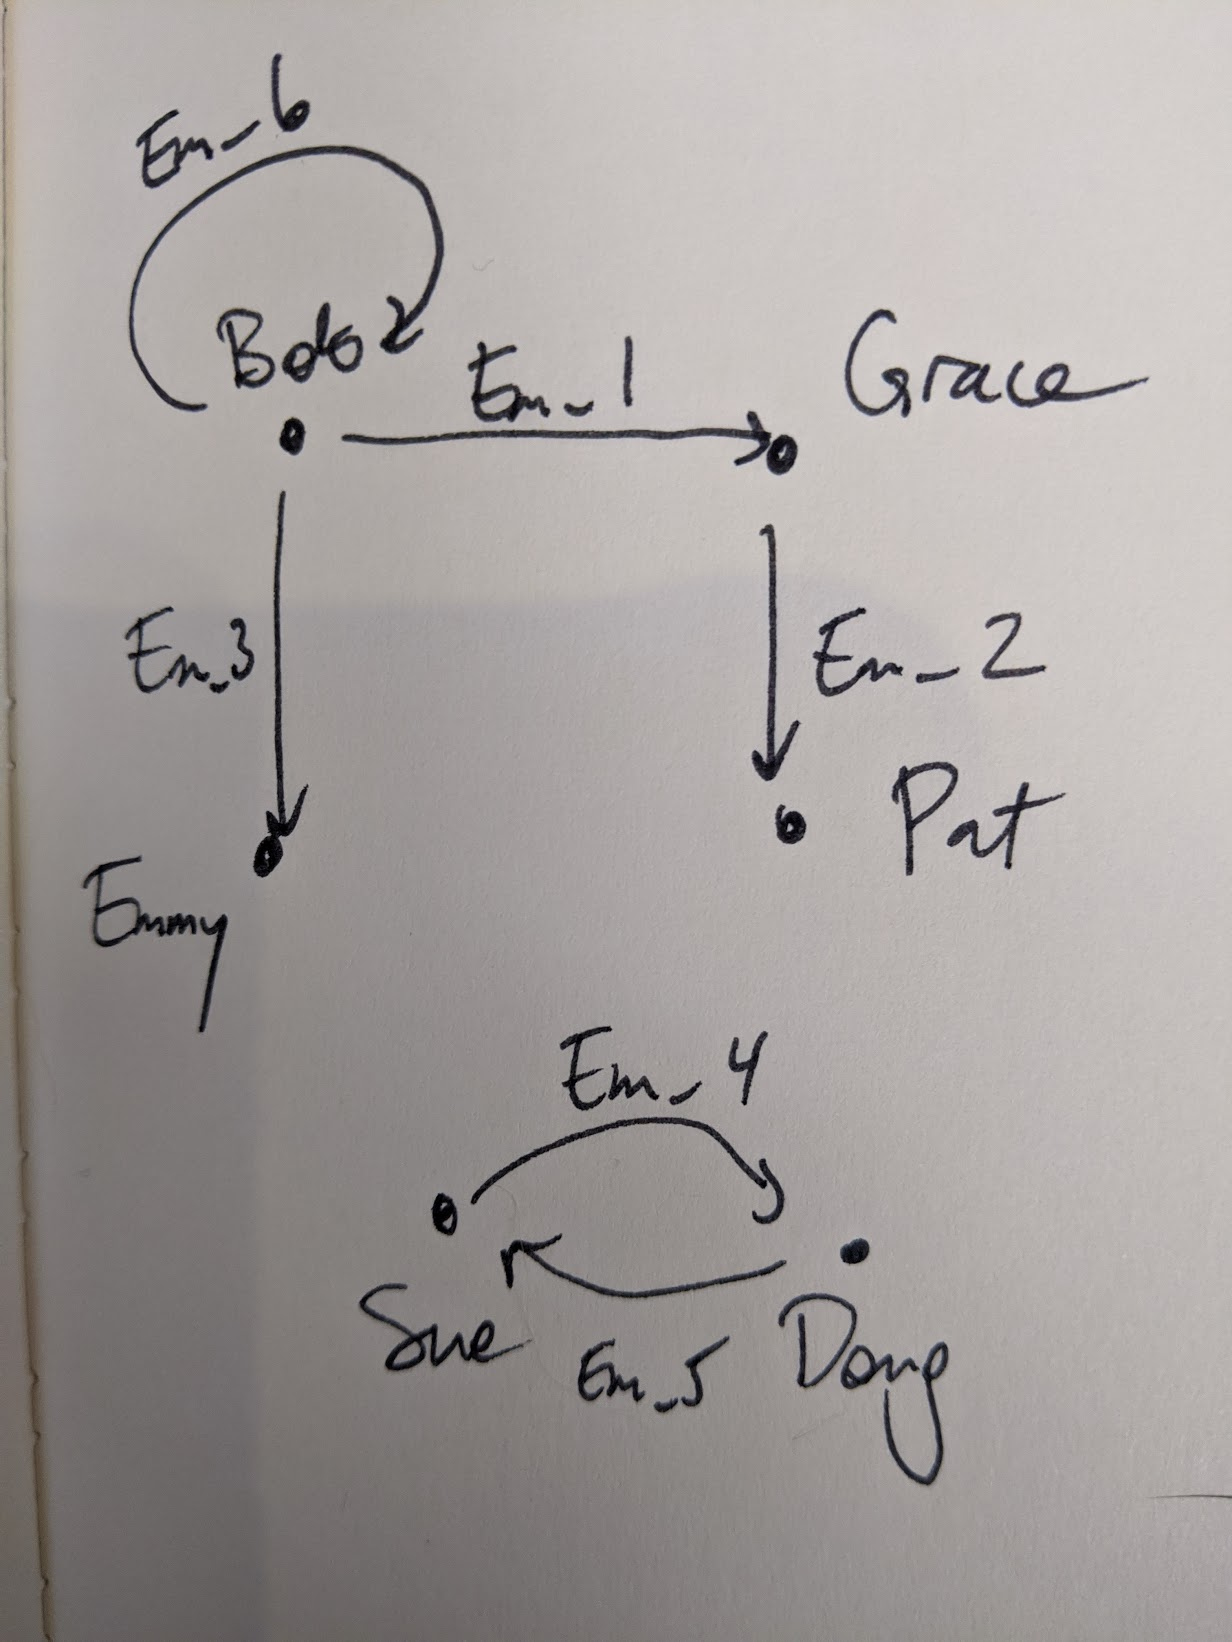
\includegraphics[width=0.5\textwidth]{images/3-78.jpg}

\exercise{3.81}
Let $(P,\leq)$ be a preorder, $z\in P$ an element and $\mcP$ the corresponding category.  Show that $z$ is a terminal object in $\mcP$ iff it is a top element in $P$: that is, for all $c\in P$ we have $c\leq z$.

\solution
By definition, we know $z$ is a terminal object if for every $c\in P$ we have a unique morphism $c\to z$.  But as there is only at most one morphism between any two objects in a preorder, namely $\leq$, this implies that $c\leq z$ for all $c\in P$.

\exercise{3.82}
Name a terminal object in $\Cat$.

\solution
Any category with a single object and a single morphism (the identity on that object) is a terminal object in $\Cat$.  This is due to Exercise 3.76.

\exercise{3.83}
Find a category that doesn't have a terminal object.

\solution
The schema $\textbf{Gr}$ from before is a category without a terminal object.  Arrow cannot be terminal as there is nor morphism from Vertex to Arrow, and Vertex cannot be terminal as there are two distinct morphisms from Arrow to Vertex.

\exercise{3.88}
Let $(P,\leq)$ be a preorder, let $x,y\in P$ be elements, and let $\mcP$ be the corresponding category.  Show that the product $x\times y$ in $\mcP$ agrees with their meet $x\land y$ in $P$.

\solution
Note that for a preorder, we need only show that a morphism exists to have a unique morphism between objects as there can only be at most one.

By definition, $x\land y \leq x,y$, which gives us the projection morphisms $p_x$ and $p_y$ in the definition of the product.  Also for any $c\in P$ where $c\leq x$ and $c\leq y$, we know that $c\leq x\land y$, giving us the unique morphism $\langle f,g\rangle$.  Hence the meet exactly corresponds to the product.

\exercise{3.90}
\begin{enumerate}
	\item What are the identity morphisms in a product category $\mcC\times\mcD$?
	\item Why is composition in a product category associative?
	\item What is the product category $\textbf{1}\times\textbf{2}$?
	\item What is the product category $\mcP\times\mcQ$ when $P$ and $Q$ are preorders and $\mcP$ and $\mcQ$ the corresponding categories?
\end{enumerate}

\solution
\begin{enumerate}
	\item The identity morphisms are just pairs of identities $(\id_c,\id_d)$ for $c\in\Ob(\mcC)$ and $d\in\Ob(\mcD)$.
	\item Composition is associative simply because the underlying composition of morphisms in $\mcC$ and $\mcD$ is associative.
	\item 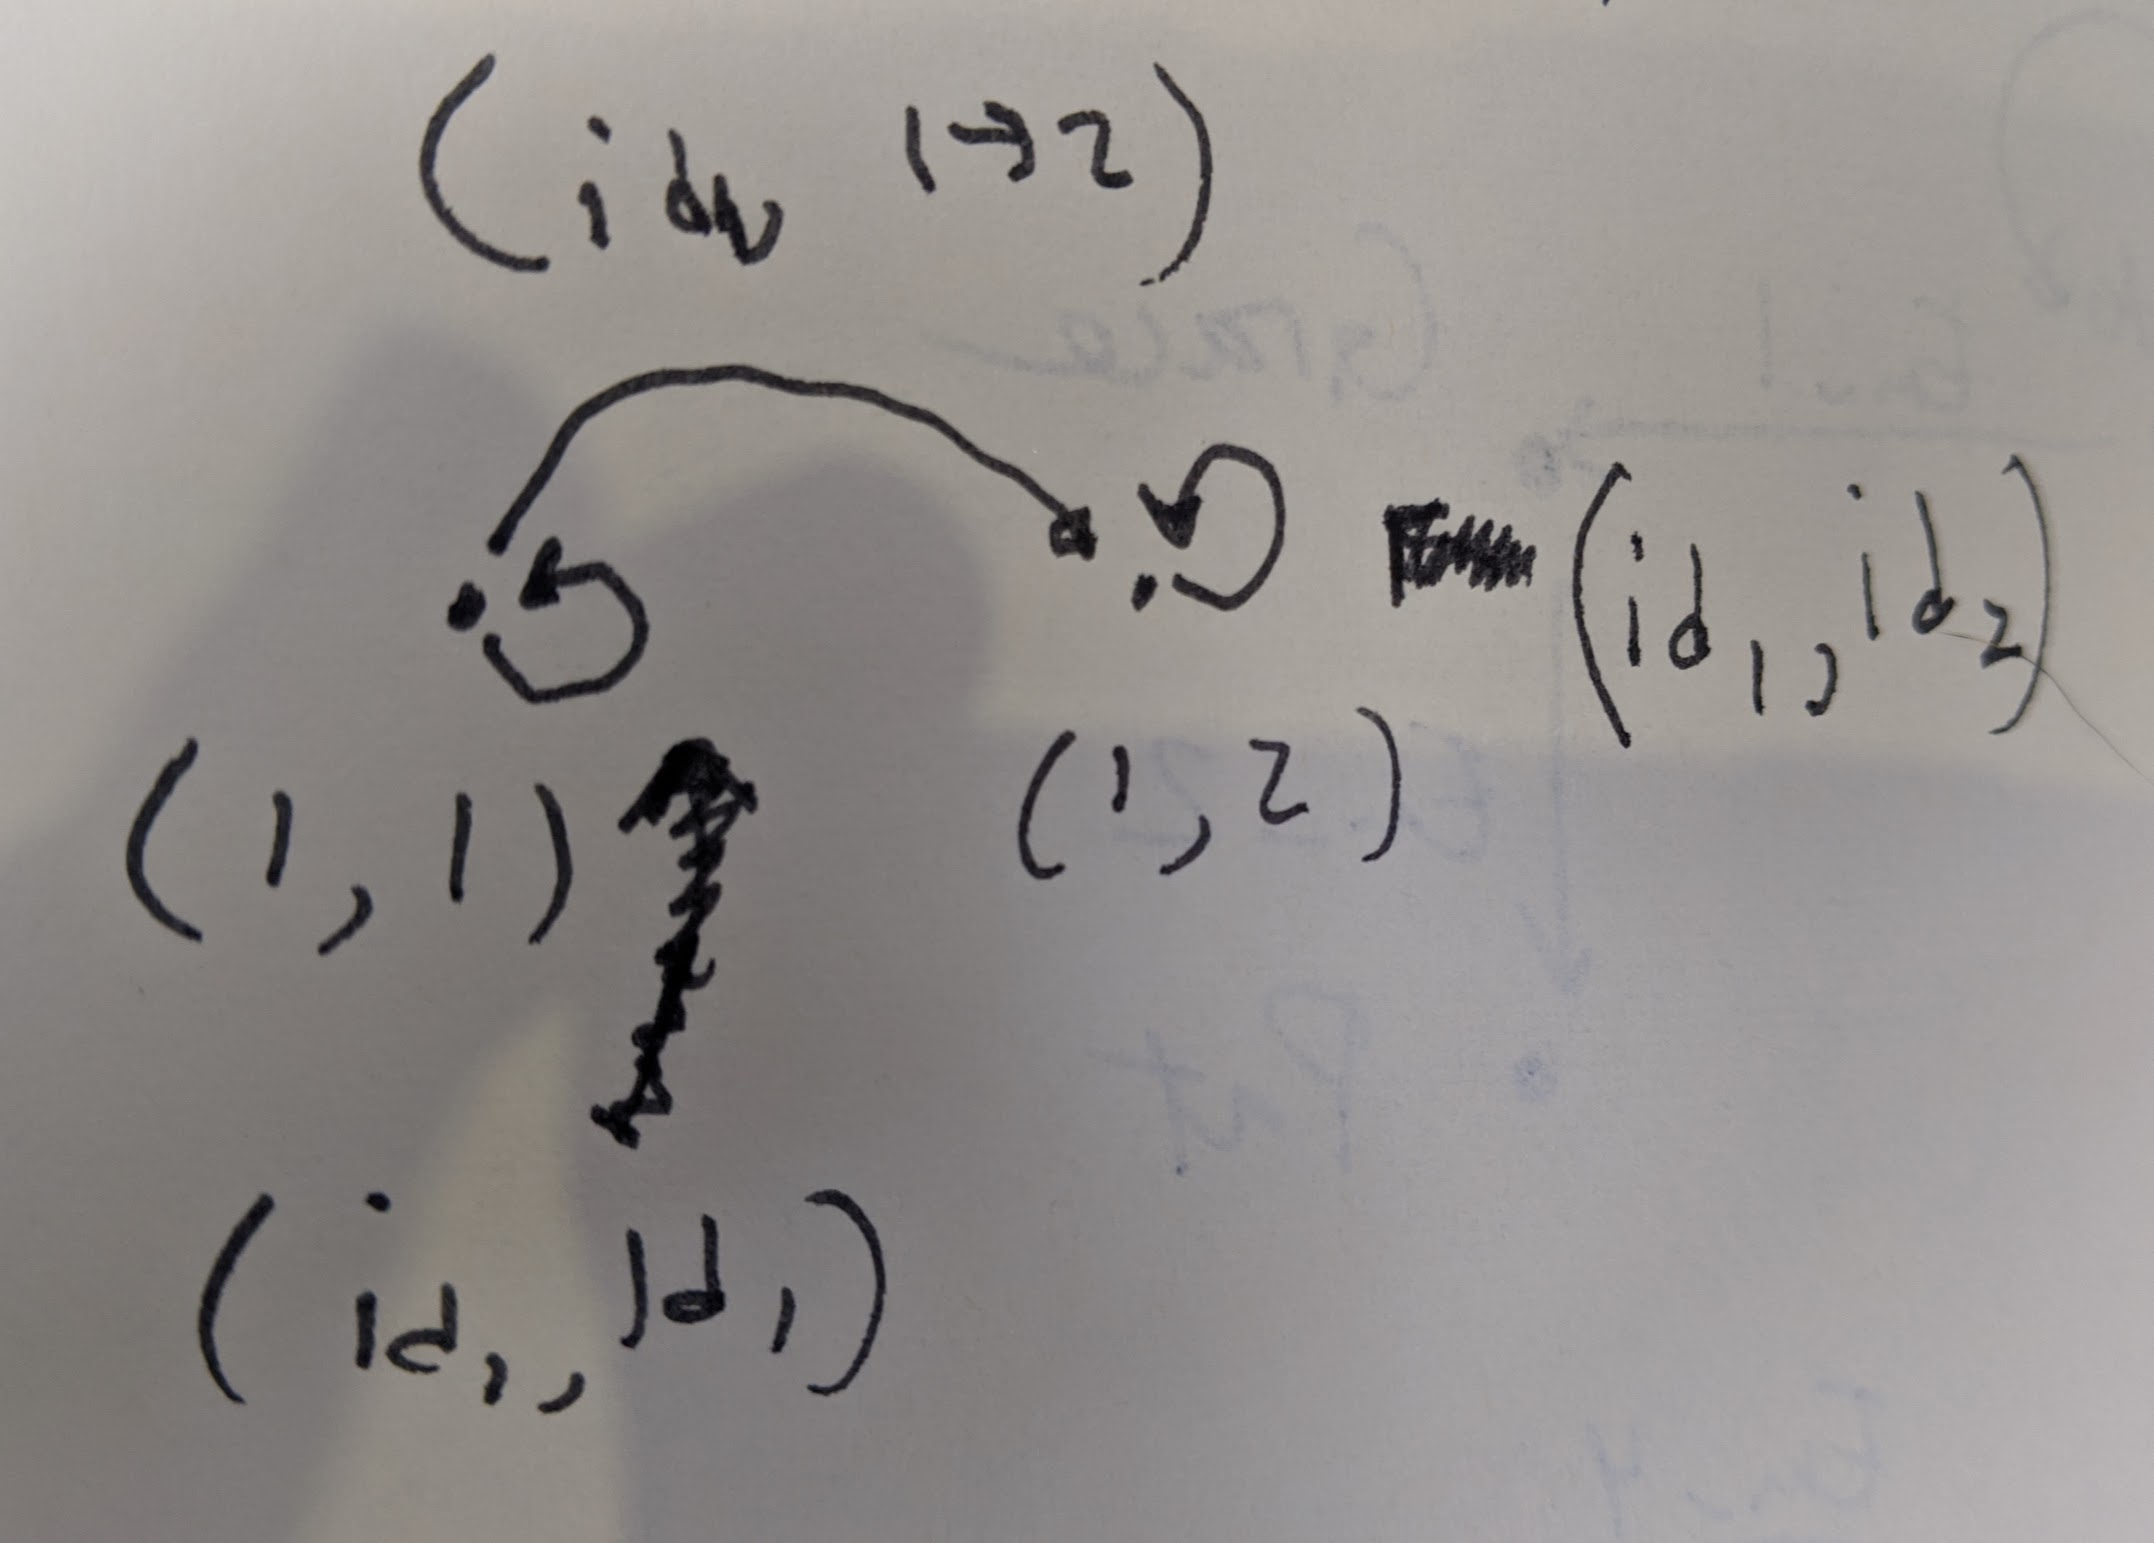
\includegraphics[width=0.5\textwidth]{images/3-90.jpg}
	\item $\mcP\times\mcQ$ has underlying set $P\times Q$ and a morphism $(p_1,q_1)\to(p_2,q_2)$ whenever $p_1\leq p_2$ and $q_1\leq q_2$.
\end{enumerate}

\exercise{3.91}
Check that a product $X\times Y$ is exactly the same as a terminal object in $\textbf{Cone}(X,Y)$.

\solution
$X\times Y$ is terminal if for every object in $\textbf{Cone}(X,Y)$, consisting of $C\in\Ob(\mcC)$ with  maps $f$ and $g$ to $X$ and $Y$ respectively, there is a unique cone morphism from $C\to X\times Y$.  But we have such a morphism from the definition of the product, namely $\langle f,g\rangle$, so $X\times Y$ is terminal.

\exercise{3.97}
Show that the limit formula in Theorem 3.95 works for products.

\solution
The product is the limit when the indexing category is just two objects and no non-identity morphisms (i.e. no arrows).  So the definition given in Theorem 3.95 gives the entire cartesian product of two sets.

\exercise{3.98}
If $D:\textbf{1}\to\Set$ is a functor, what is the limit of $D$?

\solution
Theorem 3.95 says that a limit of $D$ is just the set $D(\dot)$ where $\dot$ is the sole object in $\textbf{1}$.  We will show that any set $Z$ with a bijective function to $D(\dot)$ called $z_{\dot}$ is a terminal object in the cone category and hence a limit of $D$, which is compatible with the answer given by Theorem 3.95.

We show first that for any limit $(Z,z_{\dot})$, $|Z|\geq |D(\dot)|$.  To see this consider the cone $(D(\dot),id)$, as $(Z,z_{\dot})$ is a terminal object, there is a unique morphism $a:D(\dot)\to Z$, such that $id = a\fcmp z_{\dot}$.   As function application can only decrease the cardinality of a set we have $|\id(D(\dot)|= |(a\fcmp z_{\dot})(D(\dot)| \leq |Z|$. 

Secondly we show that for any limit $(Z,z_{\dot})$, $|Z|\leq |D(\dot)|$.  To see this suppose $(Q,q_{\dot})$ is an object in the cone category such that $|Q|> |D(\dot)|$.  As a result we must have that $q_{\dot}$ maps two elements to the same value in $D(\dot)$.  We can see two morphisms from $(Q,q_{\dot})$ to itself, the identity and the morphism which flips these two elements. 

Finally we show that for any $(Z,z_{\dot})$ which satisfies the properties above and any other object in the cone category $(C,c_{\dot})$, there exists a unique morphism from $(C,c_{\dot})$ to $(Z,z_{\dot})$.  Consider any morphism $a$, from $(C,c_{\dot})$ to $(Z,z_{\dot})$, we know by definition that $a\fcmp z_{\dot} = c_{\dot}$.  Thus as $z_{\dot}$ is invertible, we can also conclude $a = c_{\dot} \fcmp z_{\dot}^{-1}$, and it is uniquely defined by $(C,c_{\dot})$ and $(Z,z_{\dot})$.  We also note that for any $(C,c_{\dot})$ and $(Z,z_{\dot})$ this morphism exists, completing the proof.

\exercise{3.101}
Let $F:\mcC\to\mcD$ be a functor.  Define its opposite $F^{\opp}: \mcC^\opp\to\mcD^\opp$, i.e. how should it act on objects and morphisms?

\solution
$F^\opp$ should take an object $c$ in $\mcC^\opp$ (and hence also in $\mcC$) to $F(c)\in\Ob(\mcD^\opp)=\Ob(\mcD)$.

Next, for a morphism $f^\opp$ in $\mcC^\opp$, $F^\opp$ should take $f^\opp$ to $F(f)^\opp$ which we know must be a morphism in $\mcD^\opp$.



\chapter{Collaborative Design}

\exercise{4.4}
See text.

\solution
\begin{enumerate}
	\item 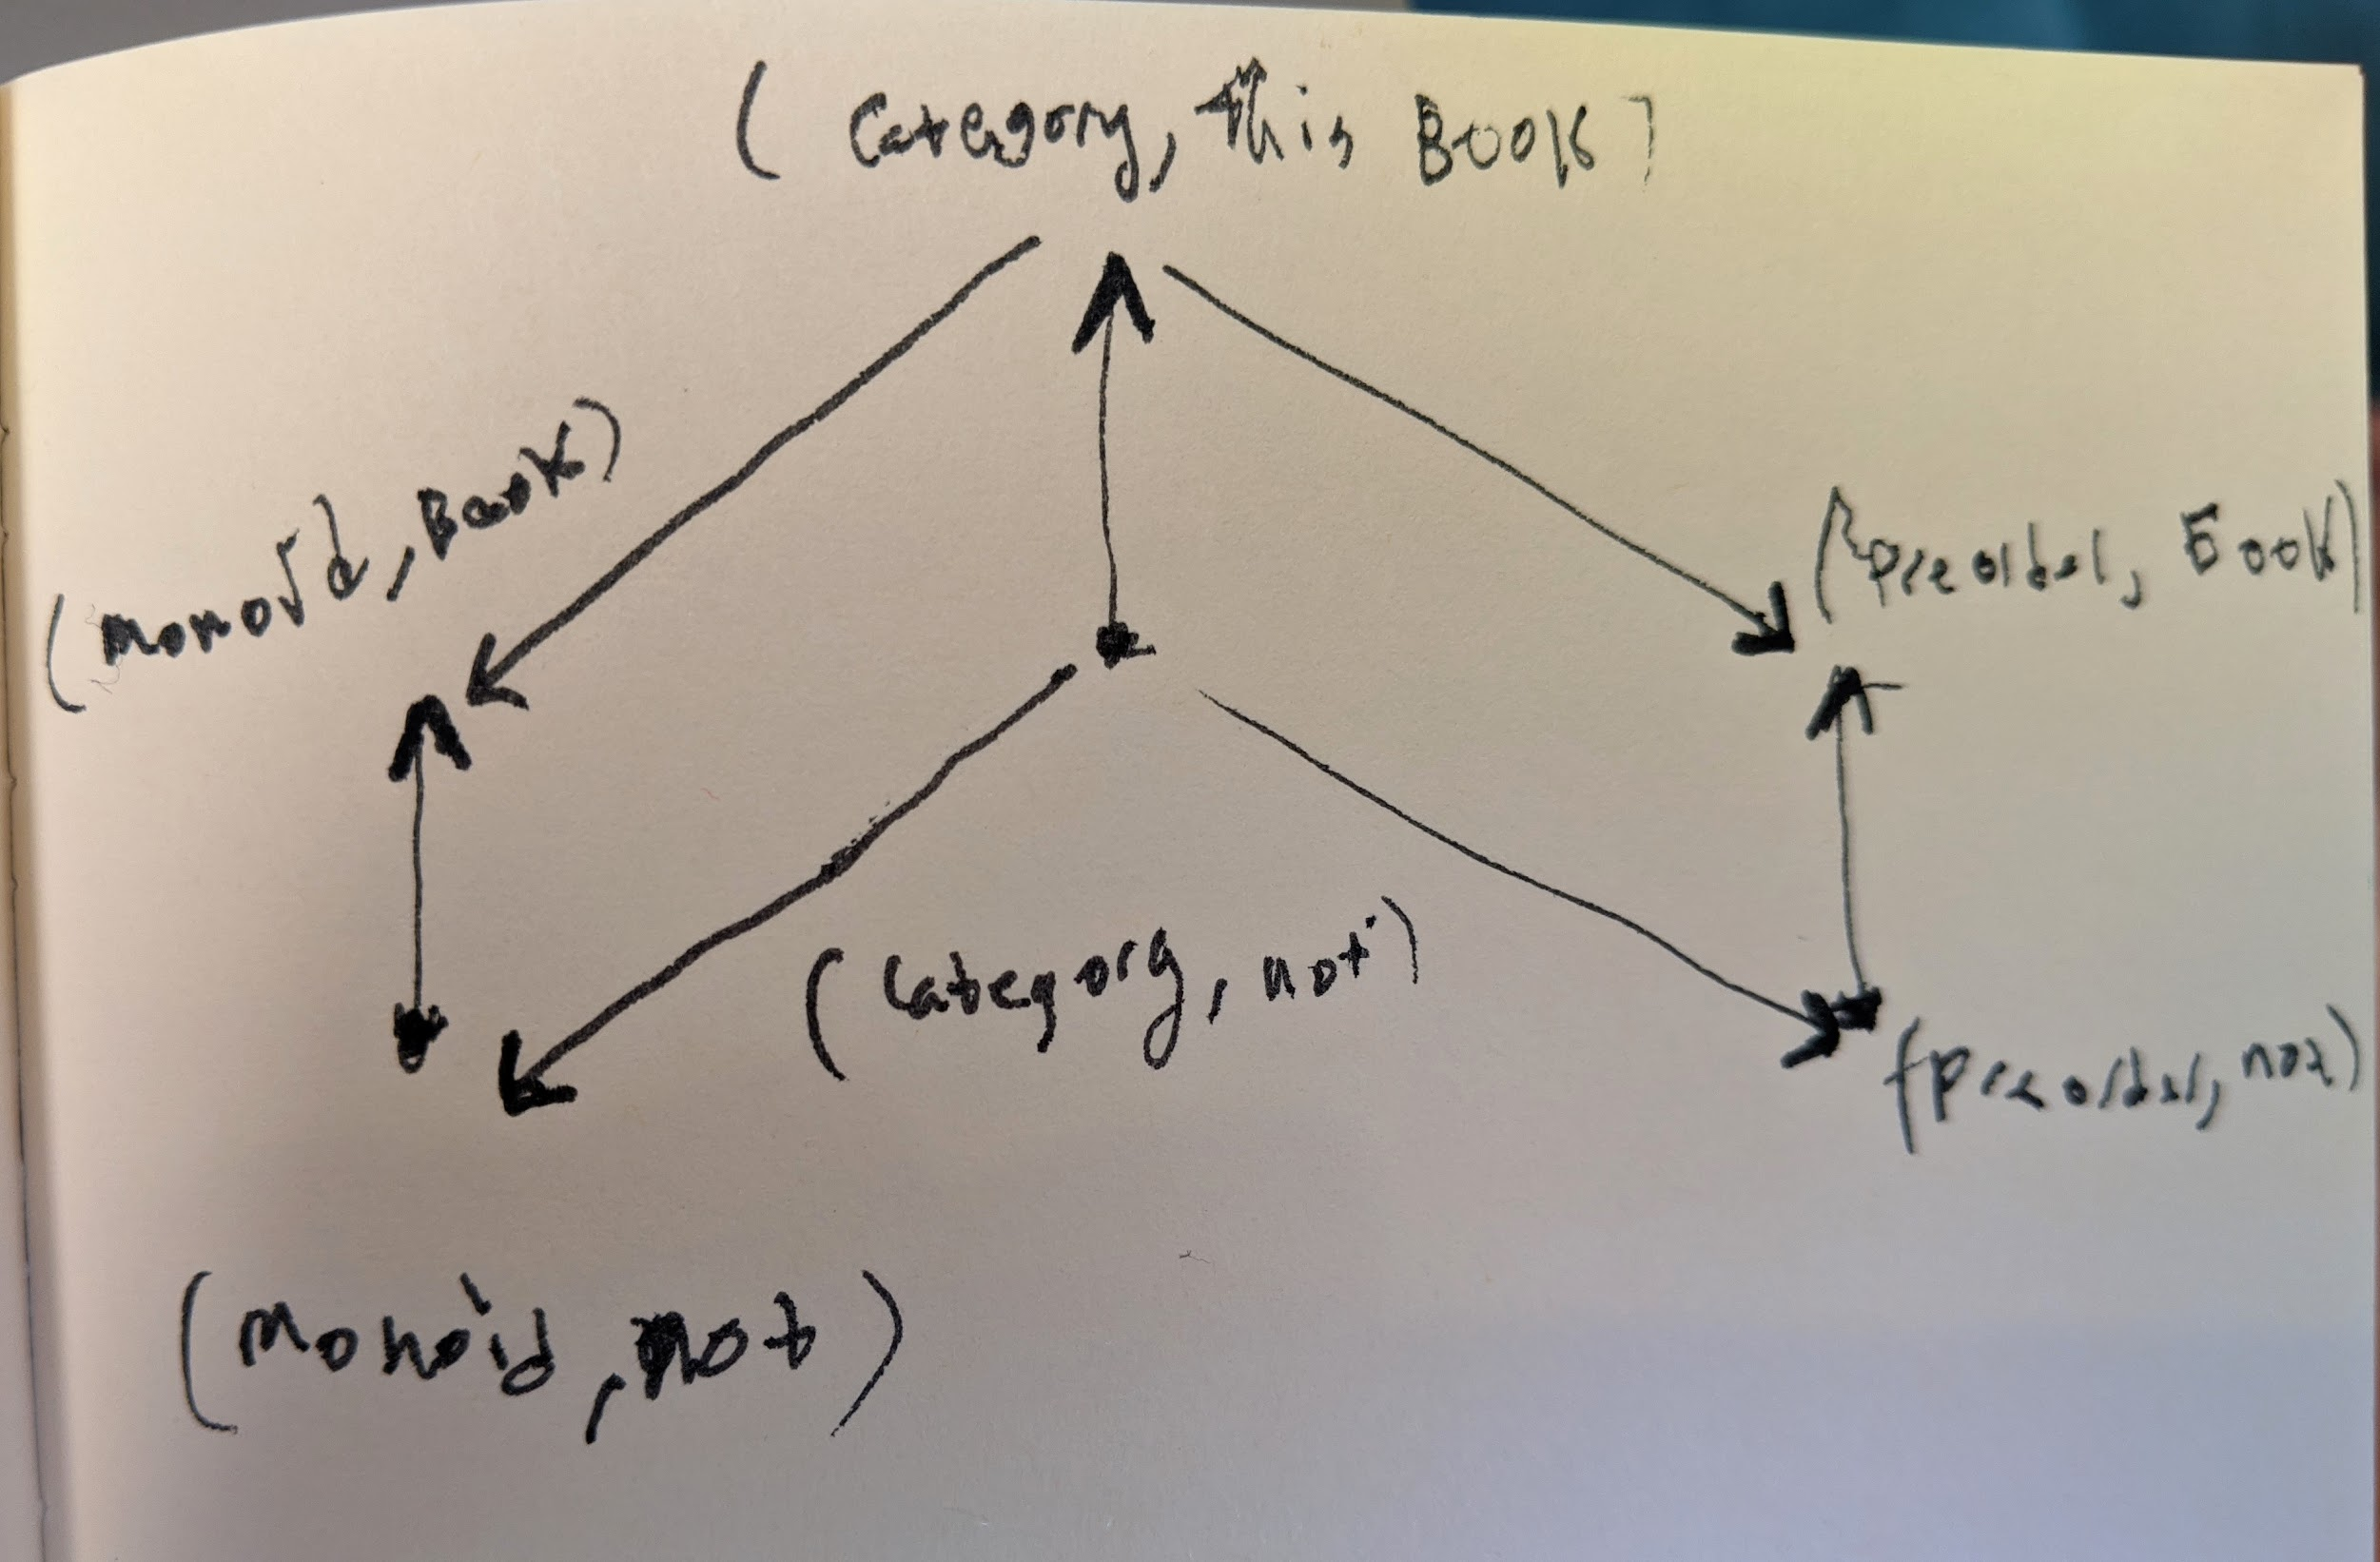
\includegraphics[width=0.5\textwidth]{images/4-4.jpg}
	\item $\Lambda(x,$ book) = true  and $\Lambda(x,$ nothing) = false for any $x\in\mcX$.
	
	  An interpretation of the fact that the preimage of true forms an upper set in $\mcX^\opp\times\mcY$ is that moving up in the product preorder corresponds to something easier, whether it is an easier topic to explain or more information to use to explain it.  So if your aunt can explain a preorder with nothing, she can definitely explain a preorder with this book, but not necessarily a category; and if she can explain a category with this book, she can definitely explain both a monoid and a preorder with this book, but not necessarily any of these topics with nothing.
\end{enumerate}

\exercise{4.7}
Discussed in person.

\exercise{4.9}
Show that a $\mcV$-profunctor is the same as a function $\Phi:\Ob(\mcX)\times\Ob(\mcY)\to V$ such that for any $x,x'\in\mcX$ and $y,y'\in\mcY$, the following holds in $\mcV$:
$$\mcX(x',x)\otimes\Phi(x,y)\otimes\mcY(y,y')\leq\Phi(x',y').$$

\solution
For a function $\Phi:\Ob(\mcX)\times\Ob(\mcY)\to \mcV$, let's use $C$ to refer to the condition \textit{for any $x,x'\in\mcX$ and $y,y'\in\mcY$, the following holds in $\mcV$:}
$$\mcX(x',x)\otimes\Phi(x,y)\otimes\mcY(y,y')\leq\Phi(x',y').$$

We first first note by the definition of a product $\mcV$-category, for any $x,x'\in\Ob(\mcX)$ and $y,y'\in\Ob(\mcY)$,
$$(\mcX^\opp\times\mcY)((x,y),(x',y'))=\mcX(x',x)\otimes\mcY(y,y')$$

So as the quantale monoid is commutative, we can see the $C$ is equivalent to \textit{for all $x,x'\in\mcX$ and $y,y'\in\mcY$, the following holds in $\mcV$:}
$$(\mcX^\opp\times\mcY)((x,y),(x',y'))\otimes\Phi(x,y)\leq\Phi(x',y').$$

Secondly we revisit the definition of a quantale enriched in itself, for $v,v'\in \mcV$ we denote $\mcV(v,v')$ as  $v\multimap v'$, and for any $t,w,v\in \mcV$
 $$(t\otimes v)\leq w \iff t\leq (v\multimap w)$$
 
Using this we can further rewrite $C$ as \textit{for all $x,x'\in\mcX$ and $y,y'\in\mcY$, the following holds in $\mcV$:}
$$(\mcX^\opp\times\mcY)((x,y),(x',y'))\leq\mcV(\Phi(x,y),\Phi(x',y')).$$

We now note this is precisely the definition of a $\mcV$-profunctor.

\exercise{4.10}
Discussed in person.

\exercise{4.12}
See text.

\solution
$$\begin{array}{c|ccccc}
\Phi & a & b & c & d & e \\
\hline N & \true & \false & \true & \false & \true \\
E & \true & \true & \false & \true & \false \\
W & \true & \false & \true & \false & \true \\
S & \true & \true & \true & \true & \true
\end{array}$$

\exercise{4.15}
See text.

\solution
$$\begin{array}{c|ccc}
\Phi & x & y & z \\
\hline A & 17 & 20 & 20 \\
B & 11 & 14 & 14 \\
C & 14 & 17 & 17 \\
D & 12 & 9 & 15
\end{array}$$

\exercise{4.17}
Calculate $M_X^3*M_\Phi*M_Y^2$, remembering to do matrix multiplication according to the $(\min,+)$-formula for matrix multiplication in the quantale $\Cost$.  Your answer should agree with the one you got in Exercise 4.15.

\solution
Discussed in person.

\exercise{4.18}
See text.

\solution
This is valid, it just means that it is not possible to make a good-natured funny movie even with \$1M, i.e. $\Phi(($g/n, funny$), $\$1M$)$ = false.

\exercise{4.22}
See text.

\solution
$$\begin{array}{c|cccc}
\Phi \fcmp \Psi & p & q & r & s \\
\hline A & 18 & 24 & 16 & 17 \\
B & 16 & 18 & 14 & 15 \\
C & 19 & 21 & 17 & 18 \\
D & 11 & 13 & 9 & 10
\end{array}$$

\exercise{4.26}
Choose a $\Cost$-category $\mcX$.  Give a bridge-style diagram for the unit profunctor $U_\mcX:\mcX\to\mcX$.

\solution
Discussed in person; there will be a bridge between each object and itself with cost 0.

\exercise{4.30}
Justify the steps in the proof of Lemma 4.27, and show which inequalities are actually equalities in the case where $\mcV=\Bool$.

\solution

\exercise{4.32}
Prove that composition of profunctors is associative.

\solution








\end{document}
